
\documentclass[10pt]{article} % For LaTeX2e
\usepackage{tmlr}
% If accepted, instead use the following line for the camera-ready submission:
%\usepackage[accepted]{tmlr}
% To de-anonymize and remove mentions to TMLR (for example for posting to preprint servers), instead use the following:
%\usepackage[preprint]{tmlr}

% Optional math commands from https://github.com/goodfeli/dlbook_notation.
%%%%% NEW MATH DEFINITIONS %%%%%

\usepackage{amsmath,amsfonts,bm}

% Mark sections of captions for referring to divisions of figures
\newcommand{\figleft}{{\em (Left)}}
\newcommand{\figcenter}{{\em (Center)}}
\newcommand{\figright}{{\em (Right)}}
\newcommand{\figtop}{{\em (Top)}}
\newcommand{\figbottom}{{\em (Bottom)}}
\newcommand{\captiona}{{\em (a)}}
\newcommand{\captionb}{{\em (b)}}
\newcommand{\captionc}{{\em (c)}}
\newcommand{\captiond}{{\em (d)}}

% Highlight a newly defined term
\newcommand{\newterm}[1]{{\bf #1}}


% Figure reference, lower-case.
\def\figref#1{figure~\ref{#1}}
% Figure reference, capital. For start of sentence
\def\Figref#1{Figure~\ref{#1}}
\def\twofigref#1#2{figures \ref{#1} and \ref{#2}}
\def\quadfigref#1#2#3#4{figures \ref{#1}, \ref{#2}, \ref{#3} and \ref{#4}}
% Section reference, lower-case.
\def\secref#1{section~\ref{#1}}
% Section reference, capital.
\def\Secref#1{Section~\ref{#1}}
% Reference to two sections.
\def\twosecrefs#1#2{sections \ref{#1} and \ref{#2}}
% Reference to three sections.
\def\secrefs#1#2#3{sections \ref{#1}, \ref{#2} and \ref{#3}}
% Reference to an equation, lower-case.
\def\eqref#1{equation~\ref{#1}}
% Reference to an equation, upper case
\def\Eqref#1{Equation~\ref{#1}}
% A raw reference to an equation---avoid using if possible
\def\plaineqref#1{\ref{#1}}
% Reference to a chapter, lower-case.
\def\chapref#1{chapter~\ref{#1}}
% Reference to an equation, upper case.
\def\Chapref#1{Chapter~\ref{#1}}
% Reference to a range of chapters
\def\rangechapref#1#2{chapters\ref{#1}--\ref{#2}}
% Reference to an algorithm, lower-case.
\def\algref#1{algorithm~\ref{#1}}
% Reference to an algorithm, upper case.
\def\Algref#1{Algorithm~\ref{#1}}
\def\twoalgref#1#2{algorithms \ref{#1} and \ref{#2}}
\def\Twoalgref#1#2{Algorithms \ref{#1} and \ref{#2}}
% Reference to a part, lower case
\def\partref#1{part~\ref{#1}}
% Reference to a part, upper case
\def\Partref#1{Part~\ref{#1}}
\def\twopartref#1#2{parts \ref{#1} and \ref{#2}}

\def\ceil#1{\lceil #1 \rceil}
\def\floor#1{\lfloor #1 \rfloor}
\def\1{\bm{1}}
\newcommand{\train}{\mathcal{D}}
\newcommand{\valid}{\mathcal{D_{\mathrm{valid}}}}
\newcommand{\test}{\mathcal{D_{\mathrm{test}}}}

\def\eps{{\epsilon}}


% Random variables
\def\reta{{\textnormal{$\eta$}}}
\def\ra{{\textnormal{a}}}
\def\rb{{\textnormal{b}}}
\def\rc{{\textnormal{c}}}
\def\rd{{\textnormal{d}}}
\def\re{{\textnormal{e}}}
\def\rf{{\textnormal{f}}}
\def\rg{{\textnormal{g}}}
\def\rh{{\textnormal{h}}}
\def\ri{{\textnormal{i}}}
\def\rj{{\textnormal{j}}}
\def\rk{{\textnormal{k}}}
\def\rl{{\textnormal{l}}}
% rm is already a command, just don't name any random variables m
\def\rn{{\textnormal{n}}}
\def\ro{{\textnormal{o}}}
\def\rp{{\textnormal{p}}}
\def\rq{{\textnormal{q}}}
\def\rr{{\textnormal{r}}}
\def\rs{{\textnormal{s}}}
\def\rt{{\textnormal{t}}}
\def\ru{{\textnormal{u}}}
\def\rv{{\textnormal{v}}}
\def\rw{{\textnormal{w}}}
\def\rx{{\textnormal{x}}}
\def\ry{{\textnormal{y}}}
\def\rz{{\textnormal{z}}}

% Random vectors
\def\rvepsilon{{\mathbf{\epsilon}}}
\def\rvtheta{{\mathbf{\theta}}}
\def\rva{{\mathbf{a}}}
\def\rvb{{\mathbf{b}}}
\def\rvc{{\mathbf{c}}}
\def\rvd{{\mathbf{d}}}
\def\rve{{\mathbf{e}}}
\def\rvf{{\mathbf{f}}}
\def\rvg{{\mathbf{g}}}
\def\rvh{{\mathbf{h}}}
\def\rvu{{\mathbf{i}}}
\def\rvj{{\mathbf{j}}}
\def\rvk{{\mathbf{k}}}
\def\rvl{{\mathbf{l}}}
\def\rvm{{\mathbf{m}}}
\def\rvn{{\mathbf{n}}}
\def\rvo{{\mathbf{o}}}
\def\rvp{{\mathbf{p}}}
\def\rvq{{\mathbf{q}}}
\def\rvr{{\mathbf{r}}}
\def\rvs{{\mathbf{s}}}
\def\rvt{{\mathbf{t}}}
\def\rvu{{\mathbf{u}}}
\def\rvv{{\mathbf{v}}}
\def\rvw{{\mathbf{w}}}
\def\rvx{{\mathbf{x}}}
\def\rvy{{\mathbf{y}}}
\def\rvz{{\mathbf{z}}}

% Elements of random vectors
\def\erva{{\textnormal{a}}}
\def\ervb{{\textnormal{b}}}
\def\ervc{{\textnormal{c}}}
\def\ervd{{\textnormal{d}}}
\def\erve{{\textnormal{e}}}
\def\ervf{{\textnormal{f}}}
\def\ervg{{\textnormal{g}}}
\def\ervh{{\textnormal{h}}}
\def\ervi{{\textnormal{i}}}
\def\ervj{{\textnormal{j}}}
\def\ervk{{\textnormal{k}}}
\def\ervl{{\textnormal{l}}}
\def\ervm{{\textnormal{m}}}
\def\ervn{{\textnormal{n}}}
\def\ervo{{\textnormal{o}}}
\def\ervp{{\textnormal{p}}}
\def\ervq{{\textnormal{q}}}
\def\ervr{{\textnormal{r}}}
\def\ervs{{\textnormal{s}}}
\def\ervt{{\textnormal{t}}}
\def\ervu{{\textnormal{u}}}
\def\ervv{{\textnormal{v}}}
\def\ervw{{\textnormal{w}}}
\def\ervx{{\textnormal{x}}}
\def\ervy{{\textnormal{y}}}
\def\ervz{{\textnormal{z}}}

% Random matrices
\def\rmA{{\mathbf{A}}}
\def\rmB{{\mathbf{B}}}
\def\rmC{{\mathbf{C}}}
\def\rmD{{\mathbf{D}}}
\def\rmE{{\mathbf{E}}}
\def\rmF{{\mathbf{F}}}
\def\rmG{{\mathbf{G}}}
\def\rmH{{\mathbf{H}}}
\def\rmI{{\mathbf{I}}}
\def\rmJ{{\mathbf{J}}}
\def\rmK{{\mathbf{K}}}
\def\rmL{{\mathbf{L}}}
\def\rmM{{\mathbf{M}}}
\def\rmN{{\mathbf{N}}}
\def\rmO{{\mathbf{O}}}
\def\rmP{{\mathbf{P}}}
\def\rmQ{{\mathbf{Q}}}
\def\rmR{{\mathbf{R}}}
\def\rmS{{\mathbf{S}}}
\def\rmT{{\mathbf{T}}}
\def\rmU{{\mathbf{U}}}
\def\rmV{{\mathbf{V}}}
\def\rmW{{\mathbf{W}}}
\def\rmX{{\mathbf{X}}}
\def\rmY{{\mathbf{Y}}}
\def\rmZ{{\mathbf{Z}}}

% Elements of random matrices
\def\ermA{{\textnormal{A}}}
\def\ermB{{\textnormal{B}}}
\def\ermC{{\textnormal{C}}}
\def\ermD{{\textnormal{D}}}
\def\ermE{{\textnormal{E}}}
\def\ermF{{\textnormal{F}}}
\def\ermG{{\textnormal{G}}}
\def\ermH{{\textnormal{H}}}
\def\ermI{{\textnormal{I}}}
\def\ermJ{{\textnormal{J}}}
\def\ermK{{\textnormal{K}}}
\def\ermL{{\textnormal{L}}}
\def\ermM{{\textnormal{M}}}
\def\ermN{{\textnormal{N}}}
\def\ermO{{\textnormal{O}}}
\def\ermP{{\textnormal{P}}}
\def\ermQ{{\textnormal{Q}}}
\def\ermR{{\textnormal{R}}}
\def\ermS{{\textnormal{S}}}
\def\ermT{{\textnormal{T}}}
\def\ermU{{\textnormal{U}}}
\def\ermV{{\textnormal{V}}}
\def\ermW{{\textnormal{W}}}
\def\ermX{{\textnormal{X}}}
\def\ermY{{\textnormal{Y}}}
\def\ermZ{{\textnormal{Z}}}

% Vectors
\def\vzero{{\bm{0}}}
\def\vone{{\bm{1}}}
\def\vmu{{\bm{\mu}}}
\def\vtheta{{\bm{\theta}}}
\def\va{{\bm{a}}}
\def\vb{{\bm{b}}}
\def\vc{{\bm{c}}}
\def\vd{{\bm{d}}}
\def\ve{{\bm{e}}}
\def\vf{{\bm{f}}}
\def\vg{{\bm{g}}}
\def\vh{{\bm{h}}}
\def\vi{{\bm{i}}}
\def\vj{{\bm{j}}}
\def\vk{{\bm{k}}}
\def\vl{{\bm{l}}}
\def\vm{{\bm{m}}}
\def\vn{{\bm{n}}}
\def\vo{{\bm{o}}}
\def\vp{{\bm{p}}}
\def\vq{{\bm{q}}}
\def\vr{{\bm{r}}}
\def\vs{{\bm{s}}}
\def\vt{{\bm{t}}}
\def\vu{{\bm{u}}}
\def\vv{{\bm{v}}}
\def\vw{{\bm{w}}}
\def\vx{{\bm{x}}}
\def\vy{{\bm{y}}}
\def\vz{{\bm{z}}}

% Elements of vectors
\def\evalpha{{\alpha}}
\def\evbeta{{\beta}}
\def\evepsilon{{\epsilon}}
\def\evlambda{{\lambda}}
\def\evomega{{\omega}}
\def\evmu{{\mu}}
\def\evpsi{{\psi}}
\def\evsigma{{\sigma}}
\def\evtheta{{\theta}}
\def\eva{{a}}
\def\evb{{b}}
\def\evc{{c}}
\def\evd{{d}}
\def\eve{{e}}
\def\evf{{f}}
\def\evg{{g}}
\def\evh{{h}}
\def\evi{{i}}
\def\evj{{j}}
\def\evk{{k}}
\def\evl{{l}}
\def\evm{{m}}
\def\evn{{n}}
\def\evo{{o}}
\def\evp{{p}}
\def\evq{{q}}
\def\evr{{r}}
\def\evs{{s}}
\def\evt{{t}}
\def\evu{{u}}
\def\evv{{v}}
\def\evw{{w}}
\def\evx{{x}}
\def\evy{{y}}
\def\evz{{z}}

% Matrix
\def\mA{{\bm{A}}}
\def\mB{{\bm{B}}}
\def\mC{{\bm{C}}}
\def\mD{{\bm{D}}}
\def\mE{{\bm{E}}}
\def\mF{{\bm{F}}}
\def\mG{{\bm{G}}}
\def\mH{{\bm{H}}}
\def\mI{{\bm{I}}}
\def\mJ{{\bm{J}}}
\def\mK{{\bm{K}}}
\def\mL{{\bm{L}}}
\def\mM{{\bm{M}}}
\def\mN{{\bm{N}}}
\def\mO{{\bm{O}}}
\def\mP{{\bm{P}}}
\def\mQ{{\bm{Q}}}
\def\mR{{\bm{R}}}
\def\mS{{\bm{S}}}
\def\mT{{\bm{T}}}
\def\mU{{\bm{U}}}
\def\mV{{\bm{V}}}
\def\mW{{\bm{W}}}
\def\mX{{\bm{X}}}
\def\mY{{\bm{Y}}}
\def\mZ{{\bm{Z}}}
\def\mBeta{{\bm{\beta}}}
\def\mPhi{{\bm{\Phi}}}
\def\mLambda{{\bm{\Lambda}}}
\def\mSigma{{\bm{\Sigma}}}

% Tensor
\DeclareMathAlphabet{\mathsfit}{\encodingdefault}{\sfdefault}{m}{sl}
\SetMathAlphabet{\mathsfit}{bold}{\encodingdefault}{\sfdefault}{bx}{n}
\newcommand{\tens}[1]{\bm{\mathsfit{#1}}}
\def\tA{{\tens{A}}}
\def\tB{{\tens{B}}}
\def\tC{{\tens{C}}}
\def\tD{{\tens{D}}}
\def\tE{{\tens{E}}}
\def\tF{{\tens{F}}}
\def\tG{{\tens{G}}}
\def\tH{{\tens{H}}}
\def\tI{{\tens{I}}}
\def\tJ{{\tens{J}}}
\def\tK{{\tens{K}}}
\def\tL{{\tens{L}}}
\def\tM{{\tens{M}}}
\def\tN{{\tens{N}}}
\def\tO{{\tens{O}}}
\def\tP{{\tens{P}}}
\def\tQ{{\tens{Q}}}
\def\tR{{\tens{R}}}
\def\tS{{\tens{S}}}
\def\tT{{\tens{T}}}
\def\tU{{\tens{U}}}
\def\tV{{\tens{V}}}
\def\tW{{\tens{W}}}
\def\tX{{\tens{X}}}
\def\tY{{\tens{Y}}}
\def\tZ{{\tens{Z}}}


% Graph
\def\gA{{\mathcal{A}}}
\def\gB{{\mathcal{B}}}
\def\gC{{\mathcal{C}}}
\def\gD{{\mathcal{D}}}
\def\gE{{\mathcal{E}}}
\def\gF{{\mathcal{F}}}
\def\gG{{\mathcal{G}}}
\def\gH{{\mathcal{H}}}
\def\gI{{\mathcal{I}}}
\def\gJ{{\mathcal{J}}}
\def\gK{{\mathcal{K}}}
\def\gL{{\mathcal{L}}}
\def\gM{{\mathcal{M}}}
\def\gN{{\mathcal{N}}}
\def\gO{{\mathcal{O}}}
\def\gP{{\mathcal{P}}}
\def\gQ{{\mathcal{Q}}}
\def\gR{{\mathcal{R}}}
\def\gS{{\mathcal{S}}}
\def\gT{{\mathcal{T}}}
\def\gU{{\mathcal{U}}}
\def\gV{{\mathcal{V}}}
\def\gW{{\mathcal{W}}}
\def\gX{{\mathcal{X}}}
\def\gY{{\mathcal{Y}}}
\def\gZ{{\mathcal{Z}}}

% Sets
\def\sA{{\mathbb{A}}}
\def\sB{{\mathbb{B}}}
\def\sC{{\mathbb{C}}}
\def\sD{{\mathbb{D}}}
% Don't use a set called E, because this would be the same as our symbol
% for expectation.
\def\sF{{\mathbb{F}}}
\def\sG{{\mathbb{G}}}
\def\sH{{\mathbb{H}}}
\def\sI{{\mathbb{I}}}
\def\sJ{{\mathbb{J}}}
\def\sK{{\mathbb{K}}}
\def\sL{{\mathbb{L}}}
\def\sM{{\mathbb{M}}}
\def\sN{{\mathbb{N}}}
\def\sO{{\mathbb{O}}}
\def\sP{{\mathbb{P}}}
\def\sQ{{\mathbb{Q}}}
\def\sR{{\mathbb{R}}}
\def\sS{{\mathbb{S}}}
\def\sT{{\mathbb{T}}}
\def\sU{{\mathbb{U}}}
\def\sV{{\mathbb{V}}}
\def\sW{{\mathbb{W}}}
\def\sX{{\mathbb{X}}}
\def\sY{{\mathbb{Y}}}
\def\sZ{{\mathbb{Z}}}

% Entries of a matrix
\def\emLambda{{\Lambda}}
\def\emA{{A}}
\def\emB{{B}}
\def\emC{{C}}
\def\emD{{D}}
\def\emE{{E}}
\def\emF{{F}}
\def\emG{{G}}
\def\emH{{H}}
\def\emI{{I}}
\def\emJ{{J}}
\def\emK{{K}}
\def\emL{{L}}
\def\emM{{M}}
\def\emN{{N}}
\def\emO{{O}}
\def\emP{{P}}
\def\emQ{{Q}}
\def\emR{{R}}
\def\emS{{S}}
\def\emT{{T}}
\def\emU{{U}}
\def\emV{{V}}
\def\emW{{W}}
\def\emX{{X}}
\def\emY{{Y}}
\def\emZ{{Z}}
\def\emSigma{{\Sigma}}

% entries of a tensor
% Same font as tensor, without \bm wrapper
\newcommand{\etens}[1]{\mathsfit{#1}}
\def\etLambda{{\etens{\Lambda}}}
\def\etA{{\etens{A}}}
\def\etB{{\etens{B}}}
\def\etC{{\etens{C}}}
\def\etD{{\etens{D}}}
\def\etE{{\etens{E}}}
\def\etF{{\etens{F}}}
\def\etG{{\etens{G}}}
\def\etH{{\etens{H}}}
\def\etI{{\etens{I}}}
\def\etJ{{\etens{J}}}
\def\etK{{\etens{K}}}
\def\etL{{\etens{L}}}
\def\etM{{\etens{M}}}
\def\etN{{\etens{N}}}
\def\etO{{\etens{O}}}
\def\etP{{\etens{P}}}
\def\etQ{{\etens{Q}}}
\def\etR{{\etens{R}}}
\def\etS{{\etens{S}}}
\def\etT{{\etens{T}}}
\def\etU{{\etens{U}}}
\def\etV{{\etens{V}}}
\def\etW{{\etens{W}}}
\def\etX{{\etens{X}}}
\def\etY{{\etens{Y}}}
\def\etZ{{\etens{Z}}}

% The true underlying data generating distribution
\newcommand{\pdata}{p_{\rm{data}}}
% The empirical distribution defined by the training set
\newcommand{\ptrain}{\hat{p}_{\rm{data}}}
\newcommand{\Ptrain}{\hat{P}_{\rm{data}}}
% The model distribution
\newcommand{\pmodel}{p_{\rm{model}}}
\newcommand{\Pmodel}{P_{\rm{model}}}
\newcommand{\ptildemodel}{\tilde{p}_{\rm{model}}}
% Stochastic autoencoder distributions
\newcommand{\pencode}{p_{\rm{encoder}}}
\newcommand{\pdecode}{p_{\rm{decoder}}}
\newcommand{\precons}{p_{\rm{reconstruct}}}

\newcommand{\laplace}{\mathrm{Laplace}} % Laplace distribution

\newcommand{\E}{\mathbb{E}}
\newcommand{\Ls}{\mathcal{L}}
\newcommand{\R}{\mathbb{R}}
\newcommand{\emp}{\tilde{p}}
\newcommand{\lr}{\alpha}
\newcommand{\reg}{\lambda}
\newcommand{\rect}{\mathrm{rectifier}}
\newcommand{\softmax}{\mathrm{softmax}}
\newcommand{\sigmoid}{\sigma}
\newcommand{\softplus}{\zeta}
\newcommand{\KL}{D_{\mathrm{KL}}}
\newcommand{\Var}{\mathrm{Var}}
\newcommand{\standarderror}{\mathrm{SE}}
\newcommand{\Cov}{\mathrm{Cov}}
% Wolfram Mathworld says $L^2$ is for function spaces and $\ell^2$ is for vectors
% But then they seem to use $L^2$ for vectors throughout the site, and so does
% wikipedia.
\newcommand{\normlzero}{L^0}
\newcommand{\normlone}{L^1}
\newcommand{\normltwo}{L^2}
\newcommand{\normlp}{L^p}
\newcommand{\normmax}{L^\infty}

\newcommand{\parents}{Pa} % See usage in notation.tex. Chosen to match Daphne's book.

\DeclareMathOperator*{\argmax}{arg\,max}
\DeclareMathOperator*{\argmin}{arg\,min}

\DeclareMathOperator{\sign}{sign}
\DeclareMathOperator{\Tr}{Tr}
\let\ab\allowbreak


\usepackage{hyperref}
\usepackage{url}

\usepackage{amsmath}
\usepackage{amsthm}
\usepackage{dsfont}
\usepackage{placeins}

\usepackage{multirow}
\usepackage{pifont}
\usepackage{adjustbox}
\usepackage{array}
\usepackage{graphicx}
\usepackage{caption}
\usepackage{float}
\usepackage{subcaption}
\usepackage{algorithm}
\usepackage{algpseudocode}

\title{Zero-Cost Proxies Fail at the Top: Insights and a Remedy}

% Authors must not appear in the submitted version. They should be hidden
% as long as the tmlr package is used without the [accepted] or [preprint] options.
% Non-anonymous submissions will be rejected without review.

\author{\name Timotée Ly-Manson \email timotee.ly-manson@imt-atlantique.fr \\
        \addr IMT Atlantique\\
        UMR CNRS 6285 Lab-STICC\\
      \AND
      \name Mathieu Léonardon \email mathieu.leonardon@imt-atlantique.fr \\
      \addr IMT Atlantique\\
        UMR CNRS 6285 Lab-STICC\\
      \AND
      \name Abdeldjalil Aissa El Bey \email abdeldjalil.aissaelbey@imt-atlantique.fr\\
      \addr IMT Atlantique\\
        UMR CNRS 6285 Lab-STICC\\
}

% The \author macro works with any number of authors. Use \AND 
% to separate the names and addresses of multiple authors.

\newcommand{\fix}{\marginpar{FIX}}
\newcommand{\new}{\marginpar{NEW}}

\def\month{MM}  % Insert correct month for camera-ready version
\def\year{YYYY} % Insert correct year for camera-ready version
\def\openreview{\url{https://openreview.net/forum?id=XXXX}} % Insert correct link to OpenReview for camera-ready version


\begin{document}


\maketitle

\begin{abstract}
Zero-cost proxies (ZCPs) have enabled low-cost Neural Architecture Search (NAS) by removing the computational overhead from model training. While there is a strong correlation between ZCPs and model performance at the scale of entire search spaces, this does not necessarily translate to guiding the search to top performing architectures. In this paper, we conduct extensive benchmarking over state-of-the-art proxies in the TransNAS-Bench-101 setting and observe that the correlation decreases dramatically when reducing the space to the best architectures. Our findings suggest that metrics cannot reach high-end architectures on their own and require a secondary metric to constrain the space. We leverage the number of parameters as a discriminator metric in the genetic framework and introduce ParaDis, a low-cost NAS algorithm that remains orthogonal to ZCP design, with no prior over the search space. Experiments on multiple benchmarks confirm that ParaDis reaches competitive performance on a diverse array of tasks.
\end{abstract}

\section{Introduction}
\label{intro}

Neural Architecture Search (NAS) has received increasing attention as it enables the design of neural network architectures without a human expert, but has long struggled to reduce its computational cost. Various methods introduced in the early days of NAS \citep{zoph2017neural, liu2018progressive} treat the performance of the candidate architectures as a label to train a predictor. These remain the gold standard for finding the best architectures \citep{white2021bananas, schrodi2023construction}, but are impractical in real-world applications due to the large computational overhead of training each candidate from scratch.

Several lines of work related to reducing the computational cost of NAS have emerged, such as one-shot NAS \citep{pham2018efficient, guo2020single, chu2021fairnas, liu2018darts} and zero-shot NAS \citep{mellor2021neural, abdelfattah2021zero}. In the latter, the training of candidate architectures is entirely foregone in favor of ad-hoc metrics - so-called zero-cost proxies (ZCPs) - that estimate the performance of the model in its freshly initialized state, using limited data over a few forward and backward passes. Methods that incorporate these proxies have achieved competitive results \citep{jiang2023meco, peng2024swap} while reducing the computational load by several orders of magnitude.

However, zero-shot NAS has yet to offer the same performance as traditional NAS. Prior work \citep{kadlecova2024surprisingly, krishnakumar2022bench} has shown that proxies, while they can provide meaningful insights at similar model sizes, are ultimately biased towards high parameter count. An exhaustive search of the NAS-Bench-201 search space \citep{dong2020bench} on the CIFAR-10 task \citep{krizhevsky2009learning} using state-of-the-art proxy MeCo \citep{jiang2023meco} reveals that the top-ranked architecture consists solely of convolutions. This suggests that widespread parameter-free architectural choices, such as skip connections, are overlooked despite their proven benefits \citep{he2015deep, orhan2017skip}.

In this work, we first investigate the behavior of ZCPs under diverse settings in the NAS-Bench201~\citep{dong2020bench}, NAS-Bench-301~\citep{siems2020bench} and TransNAS-Bench-101 benchmark \citep{duan2021transnas} and observe an over-reliance of ZCP evaluation on Spearman correlation. Indeed, while a high Spearman correlation indicates that the proxy can generally separate high-performance architectures from lesser ones, it fails to reliably distinguish between architectures of similar performance, such as in a subspace of good architectures. This suggests that on many tasks, ZCPs cannot reach top percentiles of the space unless the space is constrained, for instance, via pairing with another metric.

We argue that parameter count is a simple yet universal metric to form such a pair. Other works \citep{colin2022adeeperlook, javaheripi2022litetransformersearch} have rightfully identified the parameter count of the model to be as strong as more complex ZCPs. However, it lacks the nuance to differentiate architectural choices at similar model sizes, which makes it a lackluster metric from the NAS point of view. Instead, we propose to view parameter count as a powerful constraint over the space to isolate more suitable regions for search via an associated ZCP. Moreover, parameter count is customizable as statistics over its distribution in the space can be directly used to target specific model sizes. We leverage this observation in \underline{\textbf{Para}}meter \underline{\textbf{Dis}}tribution Shift NAS (\textbf{ParaDis}), a novel NAS method based on a genetic algorithm framework, which assigns an arbitrary ZCP to the task of exploring the space, while simultaneously constraining based on parameter count (Fig.~\ref{fig_main_method}).

Our contributions are as follows:
\begin{enumerate}
\item We benchmark existing zero-cost proxies using the Trans-NAS-Bench-101 \citep{duan2021transnas} benchmark and shed light on the shortcomings of Spearman-based ZCP evaluation. Specifically, we show that state-of-the-art proxies suffer from a drop in performance when confronted with a space of good architectures.
\item We introduce ParaDis, a genetic-based neural architecture search method that pairs ZCPs with parameter count to target good regions of the space. ParaDis is orthogonal to ZCP design, and makes no assumption about the search space.
\item We conduct extensive experiments on the NAS-Bench-201 and TransNAS-Bench-101 benchmarks to demonstrate the effectiveness of our method.
\end{enumerate}

\begin{figure}[t]
\begin{adjustbox}{width=\linewidth}
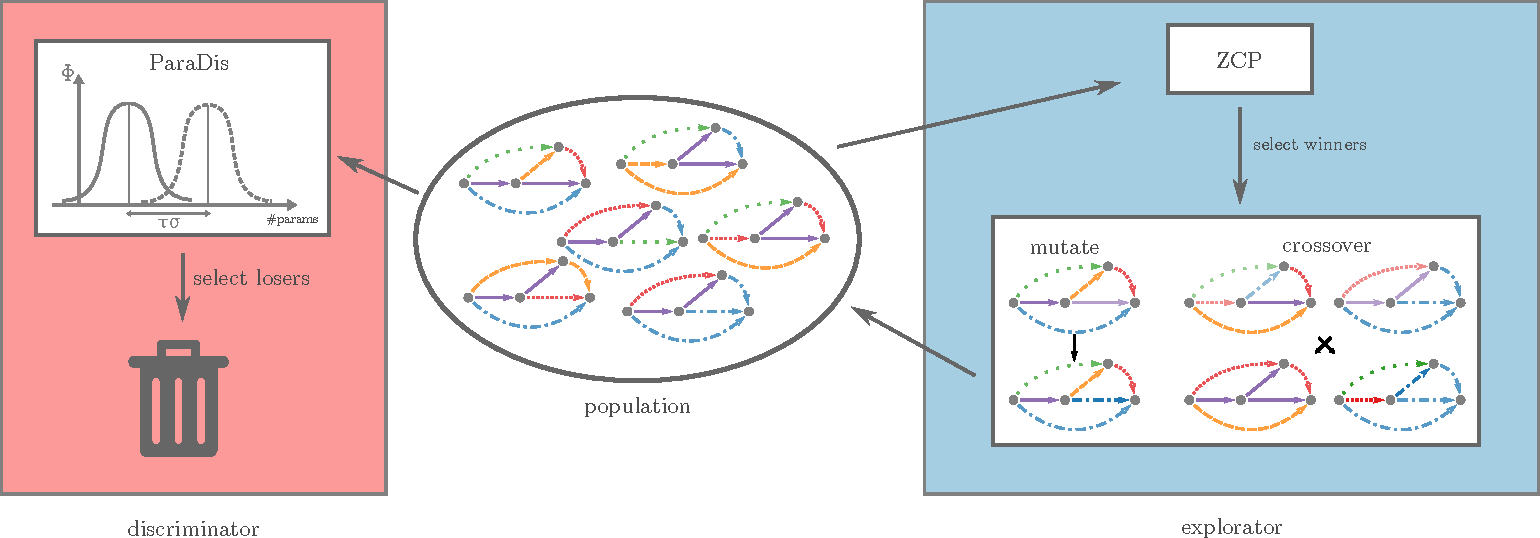
\includegraphics[width=\textwidth]{fig/paradis.pdf}

\end{adjustbox}
\caption{Our ParaDis method is based on the classic genetic zero-cost framework. Any ZCP can be used in the role of the explorer and select architectures that go on to reproduction. The ParaDis discriminator discards architectures based on parameter count distribution statistics over the population, with the size of architectures sampled at each generation controlled by $\tau$.
}
\label{fig_main_method}
\end{figure}

\section{Related works}
\label{related}

\paragraph{Zero-cost proxies} Zero-cost proxies (ZCPs) \citep{mellor2021neural, abdelfattah2021zero} hold the potential to conduct neural architecture search without the need to train architectures. A ZCP is generally derived from mathematical properties of neural networks computed from their parameters or gradients, which can be obtained during a single forward or backward pass on a batch of data. This enables the evaluation of a candidate architecture in seconds, as opposed to full retraining of the model.

Various ZCPs have been introduced for the purpose of architecture search. Initially, \citet{mellor2021neural} proposed to use the Hamming distance of the binary codes of the activations, a proxy which was later renamed \texttt{jacov}. \citet{abdelfattah2021zero} brought metrics from other fields into the NAS space. Interestingly, ZCPs tend to fall into two categories based on whether they aim to quantify the trainability of the candidate - that is, how easily it can converge to its optimal weights - or its generalization capabilities. Thus, the metrics \texttt{gradnorm}, \texttt{snip}, \texttt{graph} and \texttt{synflow} are of the trainability type, while \texttt{fisher} is of the generalization type. This observation was further explored in \citet{chen2021neural}, who paired the trainability measure \texttt{ntk}, based on the NTK condition number \citep{xiao2019disentangling}, and the expressivity measure \texttt{\#lr}, a count of the number of linear regions of the input space partitioned by the network \citep{raghu2017expressive}.

Recently, more advanced ZCPs have emerged and demonstrated competitive results on vision tasks. \texttt{zen} \citep{lin2021zen} leverages the statistics of the batch norm layers. \texttt{zico} \citep{li2023zico} exploits the link between the statistics of the gradient norms and network generalization ability. \texttt{meco} \citep{jiang2023meco} estimate convergence rate via the minimum eigenvalue of the correlation matrix. \texttt{swap} \citep{peng2024swap} reframes the question of linear regions to create a more insightful metric. While these metrics show clear theoretical merit for search space exploration, we seek to enhance their performance through the search procedure.

\paragraph{Zero-shot NAS} As ZCPs are only performance measures based on network properties, an adequate NAS algorithm is required to exploit them. Several possibilities have been explored in previous work. \citet{mellor2021neural} proposed the naive random search solution, and warm-started other traditional NAS methods with the ZCP. Similarly, \citet{abdelfattah2021zero} envisioned ZCPs as a warmup for other algorithms. \citet{chen2021neural} and \citet{jiang2023meco} implemented a pruning-like strategy where a directed acyclic graph containing all possible architectural choices is gradually pruned down to only the most desirable operation on each one of its edges. 

However, the most popular search strategy in conjunction with ZCPs remains by far the genetic approach \citep{lin2021zen, li2023zico, peng2024swap}. It is also a very common strategy for NAS in general \citep{real2018regularized, ericsson2024einspace}. Related zero-shot methods implement some form of evolution with elitist selection, meaning that ZCPs dictate which architectures are discarded from the population and which go on to mutation. In this paper, we also adopt the evolutionary framework. While other NAS methods keep the algorithmic design to a bare minimum, choosing to instead focus on the proxies' capabilities, we directly improve on the classic genetic algorithm to cover the limits of ZCPs. Importantly, this allows us to remain orthogonal to ZCP design.

\paragraph{ZCP ensembling} Intuitively, using more than one proxy should be beneficial, since metrics that evaluate different aspects of a network might cover each other's blind spots. \citet{chen2021neural} first introduced this idea by summing their \texttt{ntk} and \texttt{\#lr} metrics. \citet{he2024robustifying} generalized the idea by ensembling 6 ZCPs through weighted linear combination and learning the weights through Bayesian optimization. However, direct summation of ZCPs is impractical as the statistics of individual proxies are task-dependent and largely unknown. Without robust normalization, such sums are highly sensitive to outliers. \citet{kadlecova2024surprisingly} instead of ensemble proxies by treating them as features of the candidate architectures and applying random forest regression. Differently, we assign roles to ZCPs within the genetic framework such that they guide exploration of the search space or discriminate architectures to constrain the space.

\paragraph{Parameter count} Simply counting the parameters of a candidate architecture is a naive, yet effective proxy for accuracy. Indeed, network complexity and generalization abilities grow with network size. More often than not, the surprising effectiveness of the parameter count proxy \texttt{\#params} often discredits ZCPs \citep{colin2022adeeperlook, javaheripi2022litetransformersearch}, which are shown to be inferior to merely counting the parameters on various tasks. This metric lacks the nuance to discern common architectural choices such as the presence of skip connections, a staple of architecture design shown to improve trainability \citep{he2015deep, orhan2017skip}. Complex ZCPs might be able to identify these intricacies while failing to describe the bigger picture - which \texttt{\#params} does. 

We propose that the parameter count may serve as a prerequisite metric and adopt it as a regularizer of the search. \citet{peng2024swap} also used parameter count to regularize the score of their metric \texttt{swap} and focus the search around a desired model size. However, this requires prior knowledge of the search space's statistics which is impractical for unseen spaces where the location of good architectures in the distribution is unknown. We instead estimate the space's statistics directly from available sampled architectures, removing the need for priors over the space.

\begin{figure}[t]
\begin{adjustbox}{width=\linewidth}
    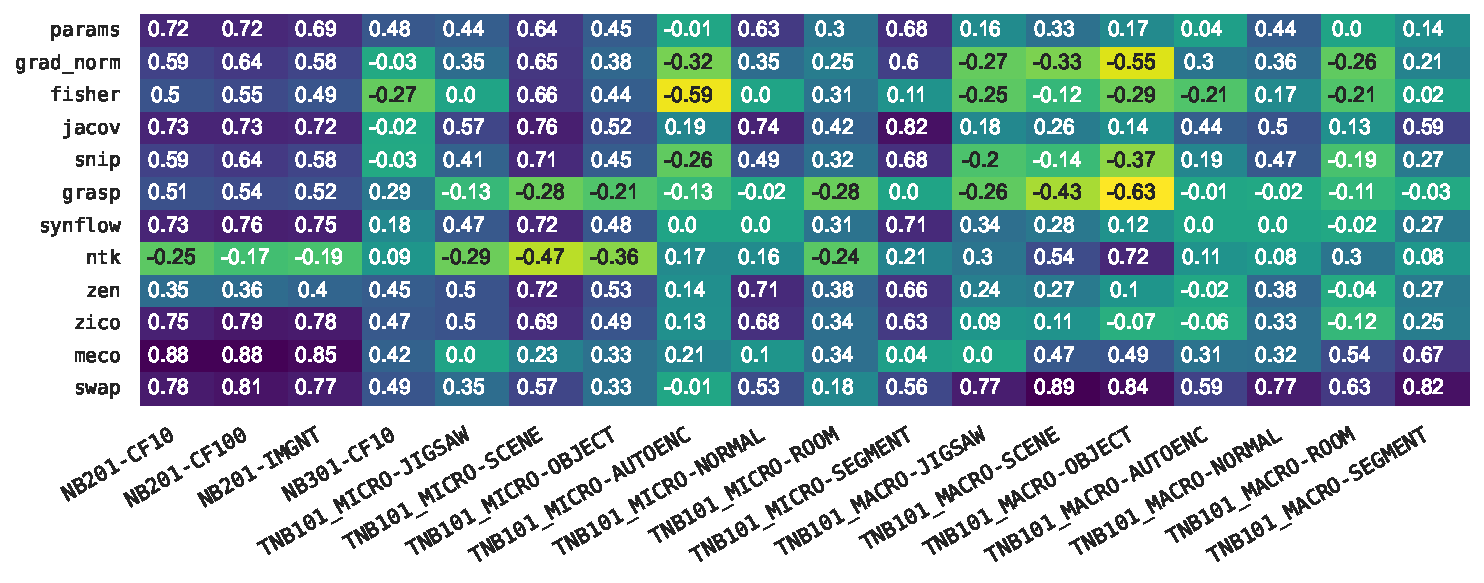
\includegraphics[width=\textwidth]{fig/benchmarks/zcp_corr.pdf}
\end{adjustbox}
\caption{\centering Spearman rank correlations of various ZCPs on the NAS-Bench-201, NAS-Bench-301 and TransNAS-Bench-101 benchmarks. Spearman was computed over 3 seeds against the entire search space.}
\label{fig_bench_corr_full}
\end{figure}

\section{Investigating the limitations of ZCPs}
\label{investigation}

\subsection{Context and benchmark description}
\label{investigation_context}

Intuitively, zero-cost proxies perform better the more correlated to actual network performance they are. In the situation of a head-to-head between several candidate architectures - the most commonplace situation for both the genetic and pruning approach in zero-shot NAS - a well-correlated metric is able to correctly choose the winner, which progresses the search in the direction of the more favorable architectures. Therefore it is without surprise that the literature has turned to benchmarking ZCPs based on their correlation to the most common search objective, validation accuracy.

A number of classic ZCPs have been benchmarked by \citet{krishnakumar2022bench} on a collection of 5 search spaces \citep{ying2019bench, dong2020bench, siems2020bench, duan2021transnas}. In this work, we consider only 4 of these search spaces:
\begin{itemize}
\item NAS-Bench-201 \citep{dong2020bench} (NB201), a cell-based space of 15625 architectures for image classification trained on CIFAR-10, CIFAR-100 and ImageNet16-120.
\item NAS-Bench-301 \citep{siems2020bench} (NB301), a search space based on DARTS \citep{liu2018darts} and evaluated on CIFAR-10 via the surrogate method.
\item TransNAS-Bench-101 Micro \citep{duan2021transnas} (TNB101-Micro), a cell-based search space of 4096 architectures tailored for diverse tasks such as object detection in the Taskonomy task bank \citep{zamir2018taskonomy} or autoencoding tasks \citep{krishnakumar2022bench}.
\item TransNAS-Bench-101 Macro \citep{duan2021transnas} (TNB101-Macro), a similar space to TNB101-Micro but focused on the macro structure with a stackable cell in 3256 different configurations.
\end{itemize}
NB201 and NB301 are designed for image classification and compatible with the common CIFAR-10, CIFAR-100 and ImageNet16-120 tasks \citep{krizhevsky2009learning, deng2009imagenet,chrabaszcz2017downsampled}, the TNB101 benchmark focuses on other paradigms and evaluating the performance of NAS across domains and tasks and outside of the classical cell-based framework.
\begin{figure}[t]
\begin{adjustbox}{width=\linewidth}
    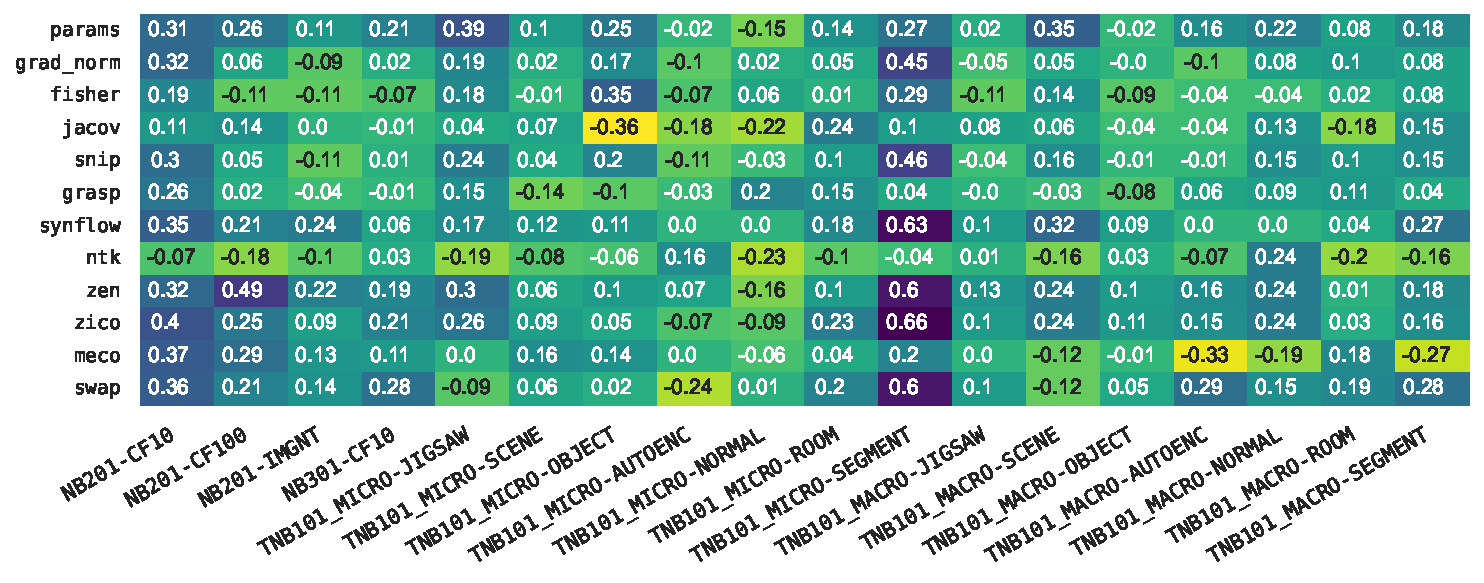
\includegraphics[width=\textwidth]{fig/benchmarks/zcp_corr_top1pct.pdf}
\end{adjustbox}
\caption{\centering Spearman rank correlations of various ZCPs on the NB201, NB301 and TNB101 benchmarks. Spearman was computed on 3 seeds against the top 1\% architectures in the space.}
\label{fig_bench_corr_top}
\end{figure}
The metric used for the benchmark is the Spearman rank correlation which is the correlation of the ranks of the ZCP scores $X$ and the ground truth scores $Y$:
$$
r_s = \frac{cov(rank(X), rank(Y))}{\sigma_{rank(X)}\sigma_{rank(Y)}}
$$
It indicates the average difference between the true rank of the candidate architecture and the rank given by the proxy. Proxies with high Spearman rank correlation tend to keep candidates ranked close to their true rank, such that a candidate is easily distinguished from others it outclasses by far.

\subsection{Benchmarking: changing the perspective}
\label{investigation_pov}

We first reproduce the benchmark proposed by \citet{krishnakumar2022bench} while including several state-of-the-art proxies that have been proposed since the initial benchmark. The results are shown in Fig.~\ref{fig_bench_corr_full}. The NAS-Bench-101 benchmark is omitted due to its large size while not providing significantly more insight than other image classification benchmarks. As we can see, newer proxies, namely \texttt{meco} and \texttt{swap}, reach high correlation on a variety of different tasks.

However, the represented search spaces are very wide and heterogeneous. We observe that on many tasks, the distributions of architecture performance in the TNB101 search spaces form distinct clusters. Therefore, high correlation over the entire search space only indicates that the proxy can eliminate all weak architectures and reach a high-performance cluster. Overall, the benchmark does not answer the central question of Neural Architecture Search: how easily can we reach the top architecture in the space?

In order to get the full picture, we adopt a novel perspective on benchmarking. For each search space, we run the benchmark restricted to only the top 1\% of architectures in the space, in terms of validation accuracy. Assuming that proxies are good enough to guide the search to the top 1\% cluster in the space, we want to assess whether they can also distinguish the performance variations in that group. The results of the benchmark are shown in Fig.~\ref{fig_bench_corr_top}. We notice a significant drop in correlation. On most tasks, none of the proxies have a correlation higher than 0.5, less than half of the correlation over the whole space. Some metrics, such as \texttt{meco} and \texttt{jacov}, show no correlation or negative correlation with the top architectures, despite having positive correlation with the entire space. Moreover, we observe that the ranking of metrics is shuffled around as metrics such as \texttt{zen} seem better suited to the top 1\% benchmark than state-of-the-art proxies for the overall benchmark, such as \texttt{meco} and \texttt{swap}.

This analysis shows that while zero-cost proxies have demonstrated the ability to weed out poorly performing architectures during the search, they cannot properly rank architectures after having reached a sub-space that contains only good candidates. Thus, considering the current state-of-the-art, there is a ceiling to the quality of architectures obtained through ZCP-driven search.

Interestingly, architectures within the same accuracy cluster, even among the top-performing ones, can differ significantly in structure. We hypothesize that using a second metric as a form of regularization of the search can constrain the search to a family of architectures that includes at least one top-performing model, and the proxy can find this architecture.

\section{ParaDis: Parameter Distribution Shifted NAS}
\label{method}

\subsection{Genetic algorithm design}
\label{method_genetic}

We introduce the ParaDis method, leveraging the genetic framework to conduct the search with a pair of metrics. For the basic genetic setup, we take inspiration from the elitist evolution algorithm proposed in \citet{peng2024swap}.

Candidate architectures are encoded into a genome in the form of a sequence of numbers, each corresponding to a possible architectural choice in the search space. While the genomes are processed and interpreted differently depending on the definition of the search space, they are processed identically within the genetic algorithm, thus decoupling search space design from the search algorithm. The various genome encodings for each search space are described in Appendix~\ref{apx_encodings}.

At first, a number of random architectures from the search space are sampled to form the initial population. As the search progresses, architectures in the population are subject to mutation and crossover operations (Fig.~\ref{fig_main_method}). During mutation, a randomly selected operation choice is transformed into another non-zero operation. Crossover is also introduced to speed up the search by enabling larger leaps in the space. Two parent architectures evenly exchange genetic material to form a child with half of its architectural choices coming from each parent.

\begin{figure}[t]
\centering
\begin{adjustbox}{width=0.74\linewidth}
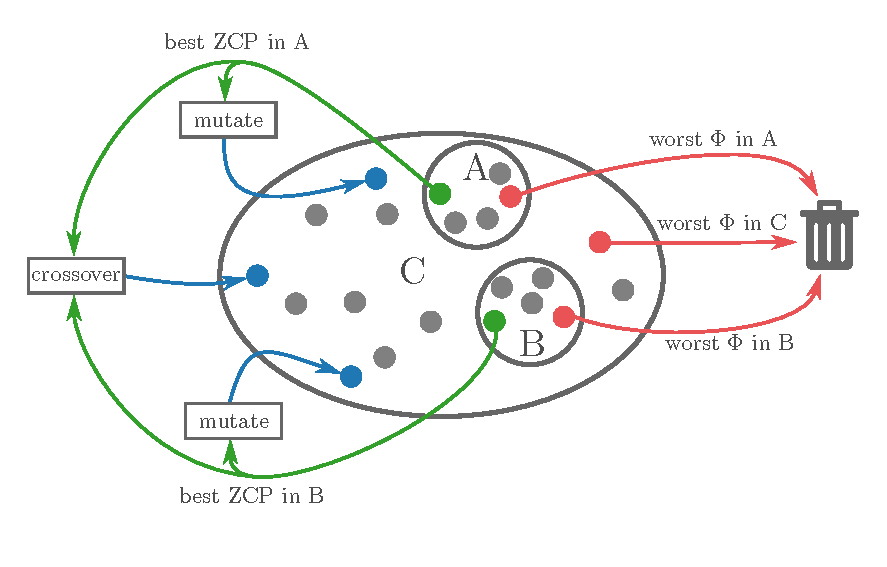
\includegraphics[width=\textwidth]{fig/details_method.pdf}

\end{adjustbox}
\caption{In the ParaDis genetic setup, architectures from the population are sampled into 3 groups. In  each group, the explorer ZCP selects parents for reproduction, while the discriminator $\Phi$ removes ill-suited architectures. At each evolution step, 3 new architectures are created and 3 are discarded.
}
\label{fig_details_method}
\end{figure}

During each evolution step, the population is divided randomly into three groups: A, B, and C. A and B are of similar size, while C is made up of all remaining architectures. Competition takes place within groups A and B, where the least fit candidates in each group are removed from the population. The most fit candidates are selected as winners: they undergo mutation and also serve as parents in the crossover operation. The resulting offspring candidate is added to the population, replacing the most unfit architecture in group C in order to maintain a constant population size. Therefore, at each evolution step, three new architectures are produced. This splitting setup introduces stochasticity to architecture selection, preventing the search from collapsing early into local optima due to the lack of genetic diversity.

We allow pairs of metrics to drive the search by assigning them two distinct roles:
\begin{itemize}
\item \textbf{Explorer} metric: directs exploration of the search by choosing competition winners, which go on to mutation and crossover. This should typically be a metric that can distinguish good architectures, even if there are false positives.

\item \textbf{Discriminator} metric: constrains the space by choosing competition losers, which are removed from the population. This should be a very reliable metric that identifies architectures to weed out in order to restrict the space to a desirable region.
\end{itemize}

While we define these roles in relation with the genetic algorithm design, the main intuition - that some metrics are better suited to choose good architectures, and others to detect bad architectures - holds across other NAS paradigms. 

Additionally, this framework is easily generalizable to the regular zero-cost setup by assuming the explorer and discriminator to be the same. However, most zero-cost proxies are designed for high-scoring architectures and are therefore more suited for the exploration role. For this reason, the explorer is flexible and can be any zero-cost proxy. This keeps the method fully orthogonal to proxy design. For the discriminator, we instead leverage the power of parameter count and introduce parameter distribution shift.

\subsection{Parameter Distribution Shift}
\label{method_parameter}

Several works have noted that the parameter count (\texttt{\#params}) is a strong baseline for zero-shot NAS \citep{colin2022adeeperlook, javaheripi2022litetransformersearch}. However, having an adequate number of parameters seems to be an obvious requirement for top architectures in the space, since those with low parameter counts are not complex enough to perform well on the tasks. On the other hand, previous works \citep{kadlecova2024surprisingly, krishnakumar2022bench} have shown that zero-cost proxies are themselves biased towards high parameter count, which provides an intuitive explanation for the results of our experiments in Section~\ref{investigation_pov}. While being biased towards higher parameter count guides the search well in general, the highest parameter count architectures are not the best, which prevents ZCPs that follow this behavior from reaching the top of the space.

Therefore, a clever use of parameter count as a discriminator is to define a score around distribution of parameter counts and target the right model size :
$$
\Phi_\alpha = e^{-(\frac{p(\alpha) - \mu}{\sigma})^2}
$$
where $p(\alpha)$ is the parameter count of the considered architecture, $\mu$ and $\sigma$ are hyperparameters for calibration.

Interestingly, \citet{peng2024swap} used this score to directly regularize their zero-cost proxy. However, due to the complete uncertainty over what kind of distribution parameters accurately represent the space, they chose $\mu$ and $\sigma$ based on knowledge of the search space, which is unavailable in real-world contexts of NAS in unknown search spaces. Instead, we infer the parameters directly from the population's mean and standard deviation at the current generation, allowing the method to remain completely agnostic to the search space.

At the beginning of the search, encouraging the exploration of high-parameter-count architectures promotes population diversity. Toward the end, this bias is gradually reduced to favor architectures with lower parameter counts. To achieve this, the mean of the score distribution is adjusted according to a temperature-controlled schedule. The final score is computed as follows:

$$
\Phi_{\alpha, \Pi}(\tau) = e^{-(\frac{p(\alpha) - (\hat{\mu}(\Pi) + \tau\hat{\sigma}(\Pi))}{\hat{\sigma}(\Pi)})^2}
$$
where $\hat{\mu}(\Pi)$ and $\hat{\sigma}(\Pi)$ are the estimated mean and standard deviation over population $\Pi$, and $\tau$ varies from $\tau_{max}$ to $\tau_{min}$ during the search, both of which are search space-agnostic. The full genetic algorithm with parameter distribution shifted discriminator is detailed in algorithm Alg.~\ref{alg_paradis}.

\subsection{Architecture selection}
\label{method_selection}

A key drawback of the genetic solution is its inability to produce a single architecture at the end of the search. In this section we propose a possible approach to tackle this issue. Under the assumption that following the search the space has been reduced to a very small number of candidate architectures, it becomes reasonable to train some of the candidates. Indeed, it is standard practice in NAS methods to retrain the obtained candidate architecture from scratch, therefore training counts slightly higher than 1 rather cost-efficient. 

We propose to conduct the final selection of the candidates with successive halving \citep{hu2022generalizing, li2018hyperband, jamieson2016non}. All candidates are trained jointly and at fixed milestones during the training, the bottom half of architectures is dropped until only one remains, which is trained to the max number of epochs to obtain the final, trained network. Considering a 600 epochs training, with a hypothetical milestone schedule in epochs such as $[10, 20, 50, 200]$ for a population of 25 architectures as in \ref{experiments_nbsz}, the total cost of successive halving is 1400 epochs or 2.3 trainings.

Previous work \citep{ly2024analyzing} has shown that validation accuracy is an unreliable metric for pruning networks in successive halving setups due to its inherent variability. Therefore, we propose to instead discard architectures at the given schedule based on the aggregated sum of all validation accuracies since training start, which is less volatile.

\section{Experiments}
\label{experiments}

\begin{figure}[h]
\centering
\caption{Rank of best architecture in genetically evolved populations, on 8 different benchmark tasks and 10 ZCPs. We observe significant gains with a carefully designed discriminator.}
\begin{adjustbox}{width=\linewidth}
    \begin{subfigure}[t]{.51\textwidth}
        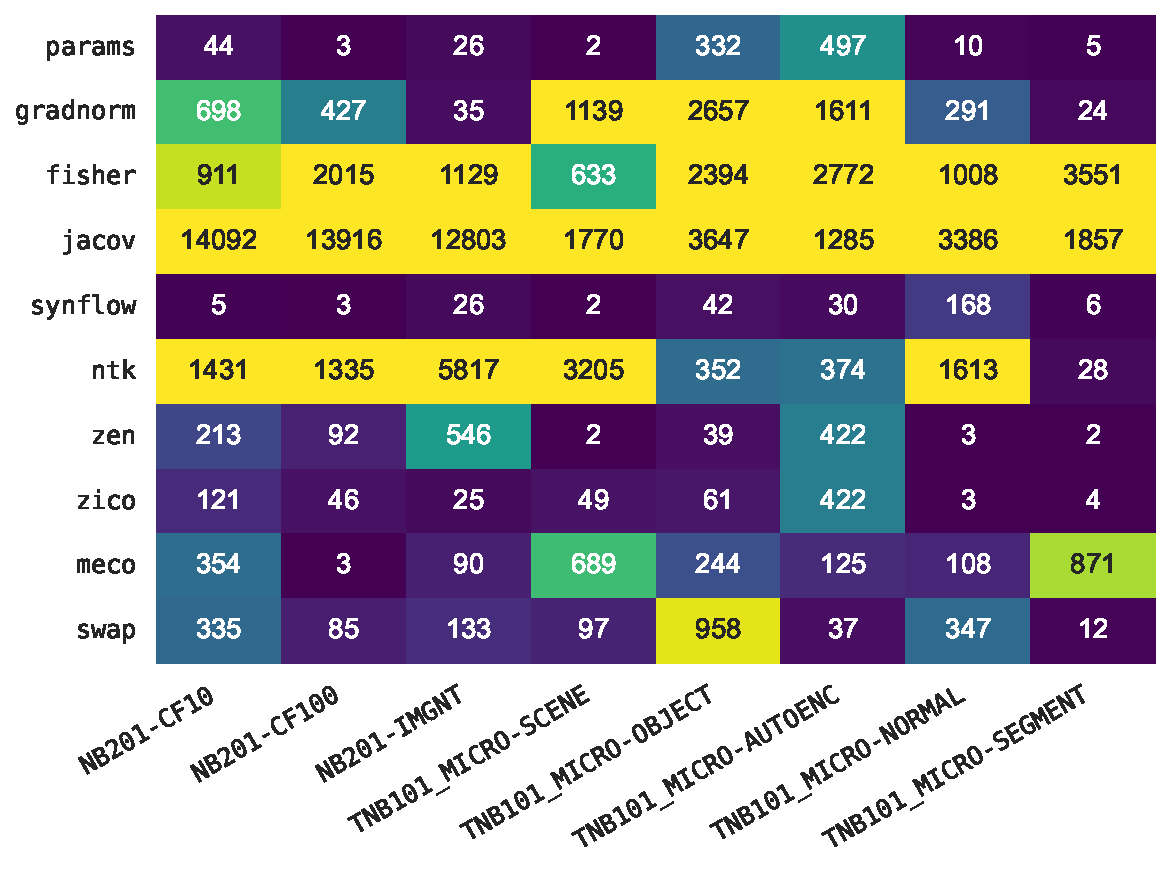
\includegraphics[width=\textwidth]{fig/exp/p2same_max_acc.pdf}
        \caption{\centering Genetic algorithm with a single ZCP}
        \label{fig_genetic_same}
    \end{subfigure}%
    \hfill%
    \begin{subfigure}[t]{.47\textwidth}
        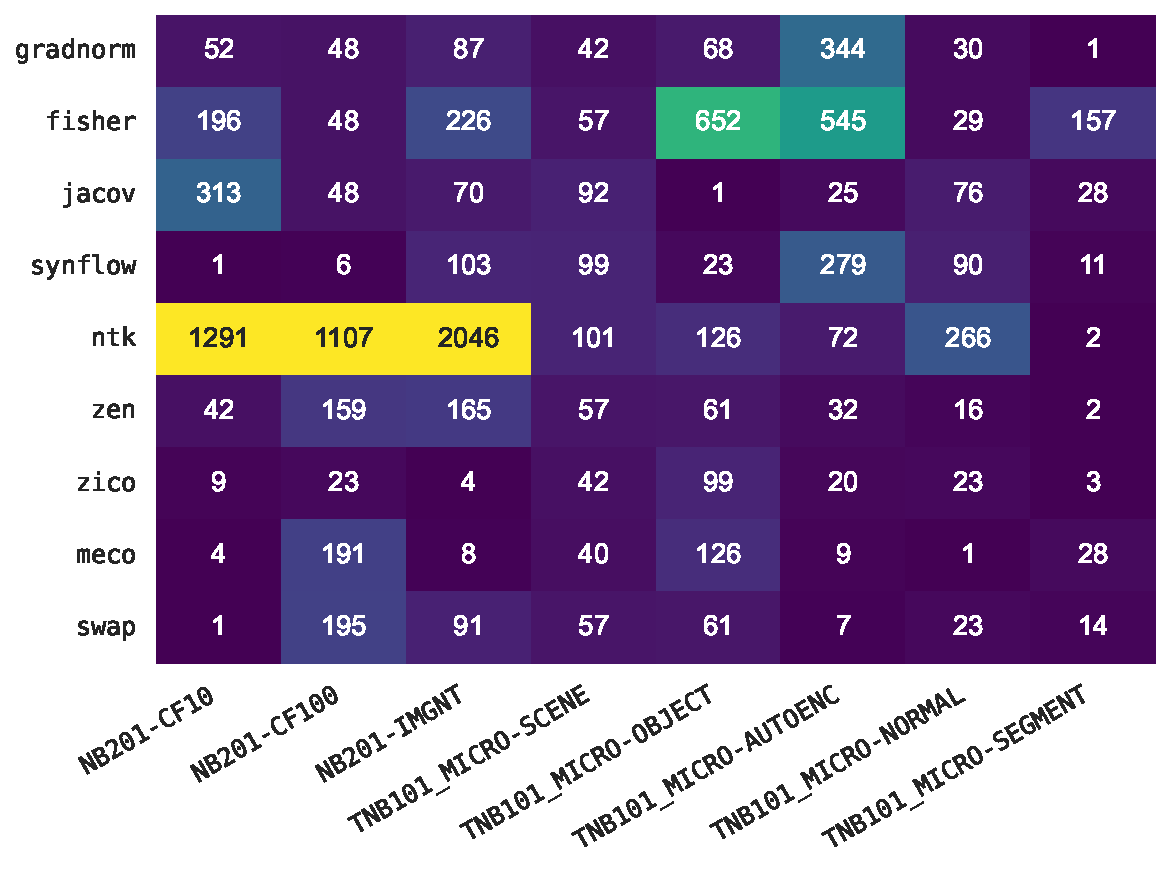
\includegraphics[width=\textwidth]{fig/exp/p2regparam_max_acc.pdf}
        \caption{\centering Genetic algorithm with ZCP explorer \\
        and parameter-based discriminator}
        \label{fig_genetic_regparams}
    \end{subfigure}%
    
\end{adjustbox}
\label{fig_genetic}
\end{figure}

\subsection{Benchmark}
\label{experiments_nbsz}

We apply our ParaDis method to the benchmarks described in \ref{investigation_context}, specifically 8 tasks from the NB201 and TNB101-Micro search spaces. We use the following hyperparameters for the genetic algorithm: population size 25, sample size of 8, 10 generations with 5 evolutionary steps per generation, totaling 50 evolution steps. For the ZCP evaluation, we set the batch size to 32 for the architectures.. On a single NVIDIA A100 GPU, the running time of our method varies between 3 and 40 minutes depending on the task and the paired proxy. We report the ranks of the best architectures in the final populations for each search space and task in Fig.~\ref{fig_genetic_regparams}. For the sake of comparison, we run our genetic algorithm as a regular zero-cost method (i.e, the discriminator metric is the same as the explorer's) using the same hyperparameters and report the results in Fig.~\ref{fig_genetic_same}.

We observe a significant boost in the quality of architectures searched with the ParaDis discriminator compared to the single ZCPs. Specifically, the ranks of discovered architectures is lower on average for every metric, and the top-ranked architecture in the space is discovered for several metric/task pairs. Unsurprisingly, the biggest gains are obtained for ZCPs that struggle to reach a good region of the space on their own: on all tasks in the NB201 space, metrics such as \texttt{fisher} and \texttt{jacov} reach the top 2\% of the search space. Overall, our benchmark experiments demonstrate that our parameter-based discriminator scheme restricts the search space to a sufficiently good region for all ZCPs to thrive.

\begin{figure}[h]
\begin{adjustbox}{width=\linewidth}

    \centering
    \begin{subfigure}[b]{.33\textwidth}
        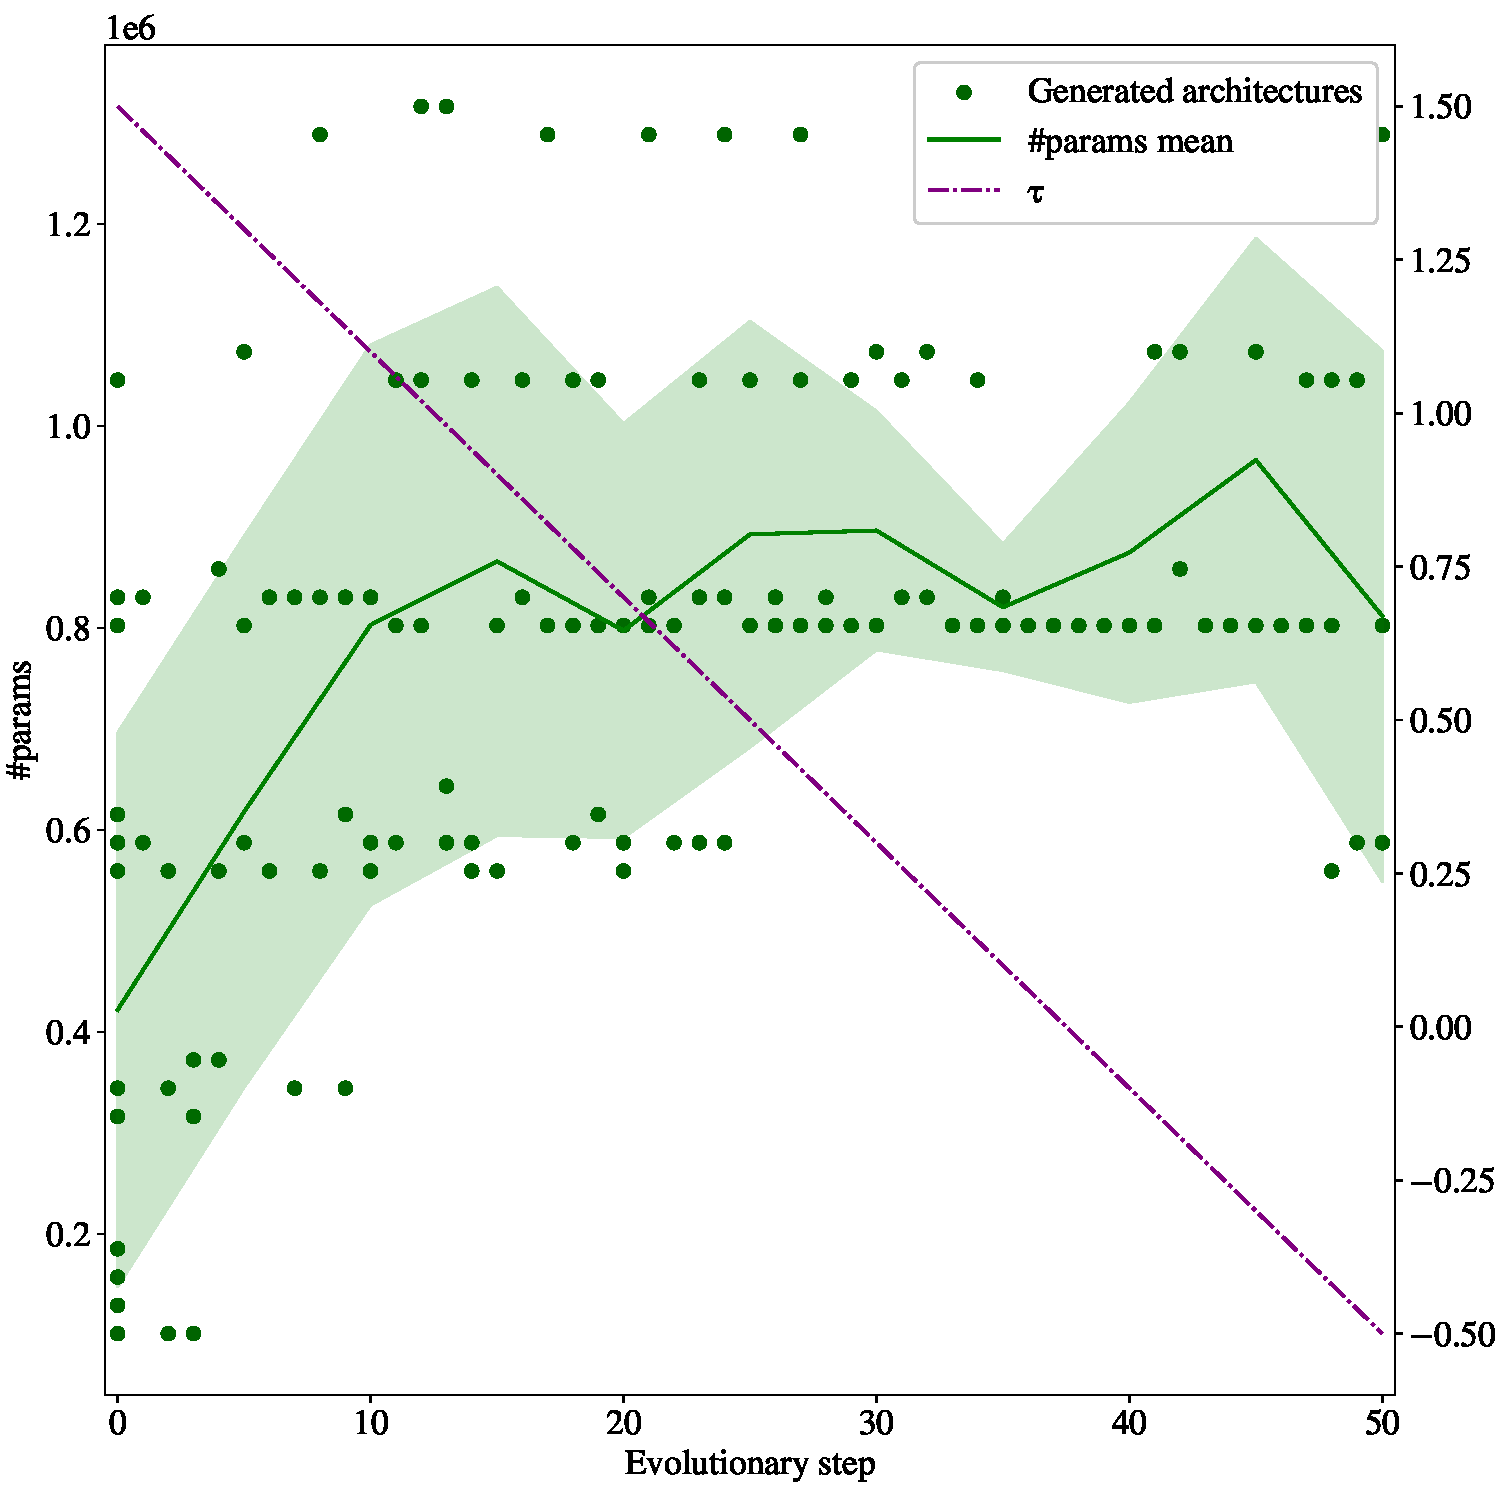
\includegraphics[width=\textwidth]{fig/params/params_adv_genetic_regparam_nasbench201_cifar10_meco_2025-04-30_16-45.pdf}
        \caption{CIFAR10}
        \label{fig_params_meco_cifar10}
    \end{subfigure}%
    \hfill%
    \begin{subfigure}[b]{.33\textwidth}
        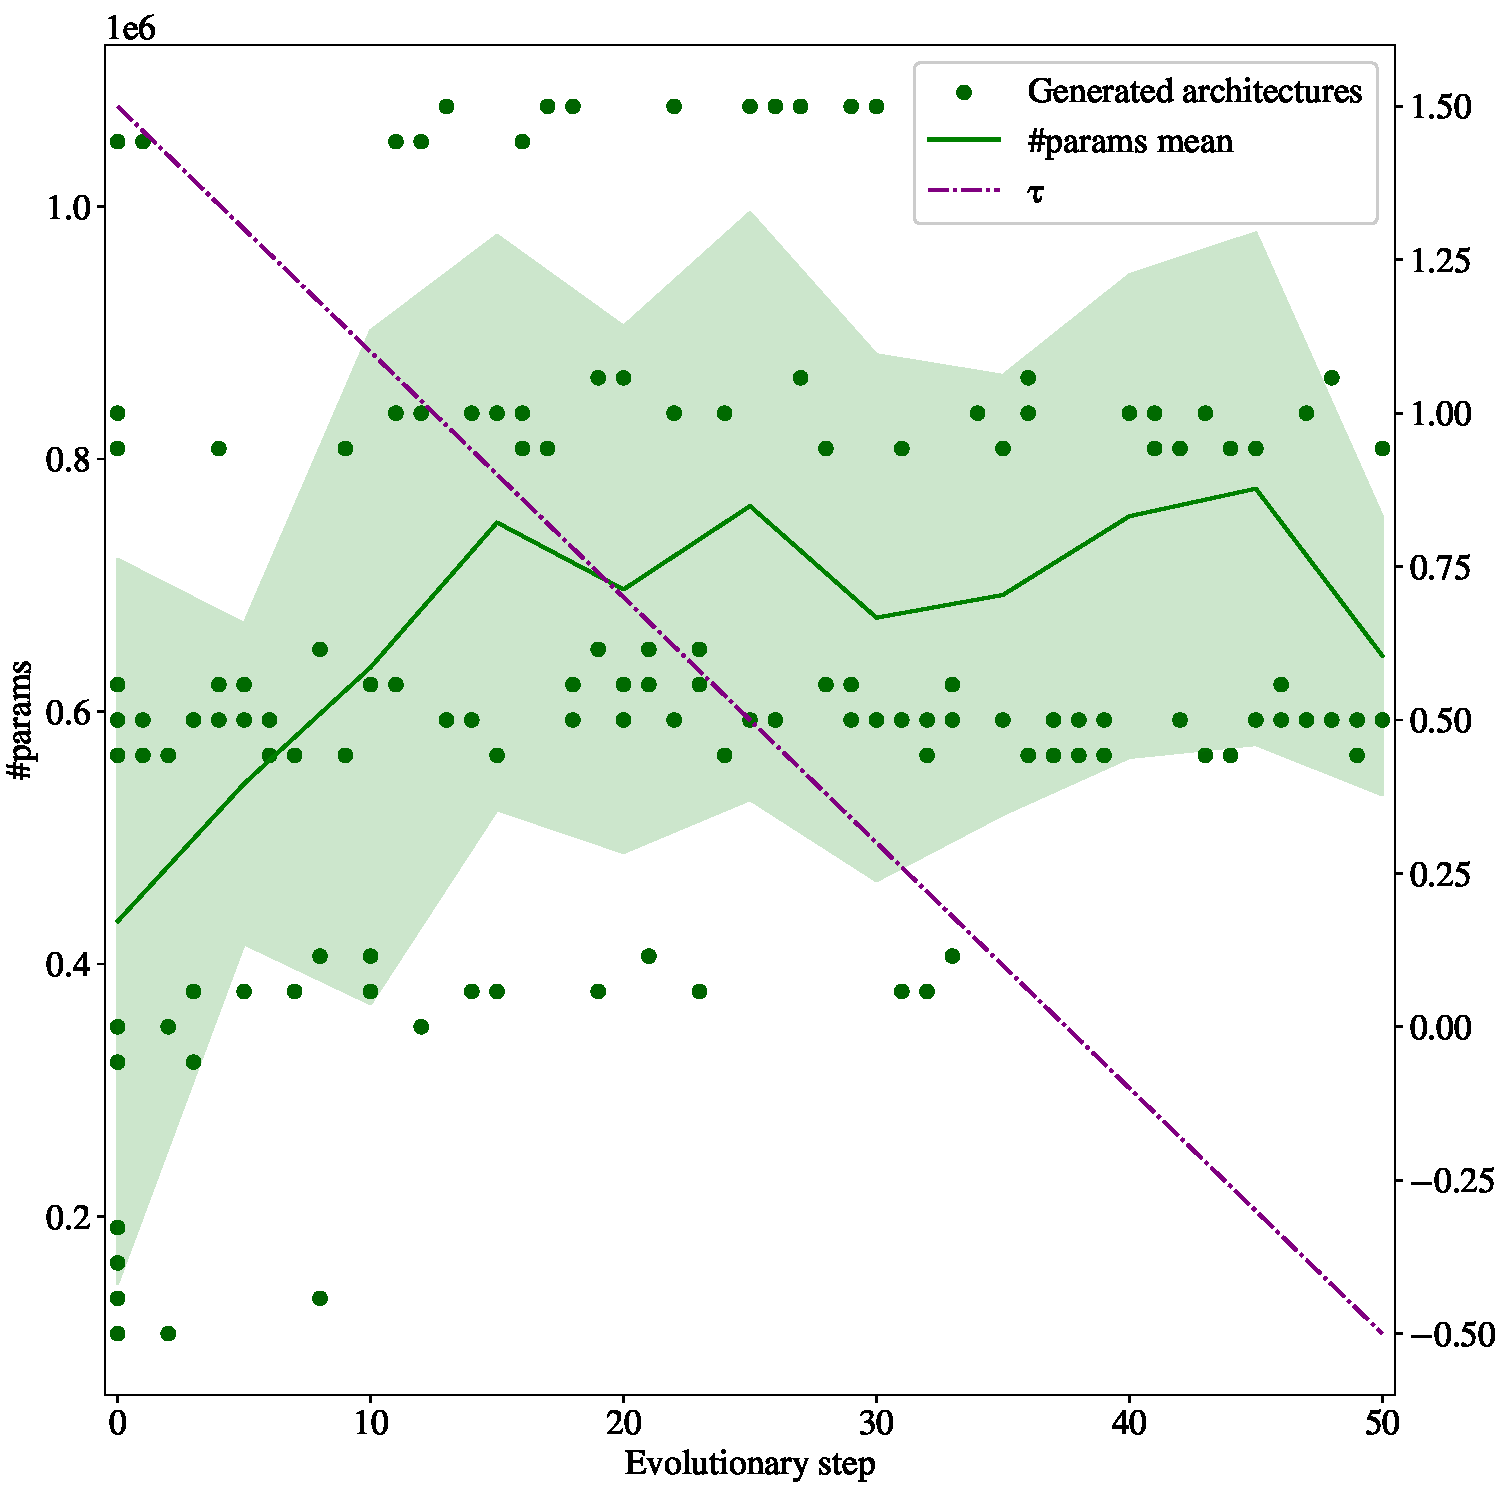
\includegraphics[width=\textwidth]{fig/params/params_adv_genetic_regparam_nasbench201_cifar100_meco_2025-04-30_16-45.pdf}
        \caption{CIFAR100}
        \label{fig_params_meco_cifar100}
    \end{subfigure}%
    \hfill%
    \begin{subfigure}[b]{.33\textwidth}
        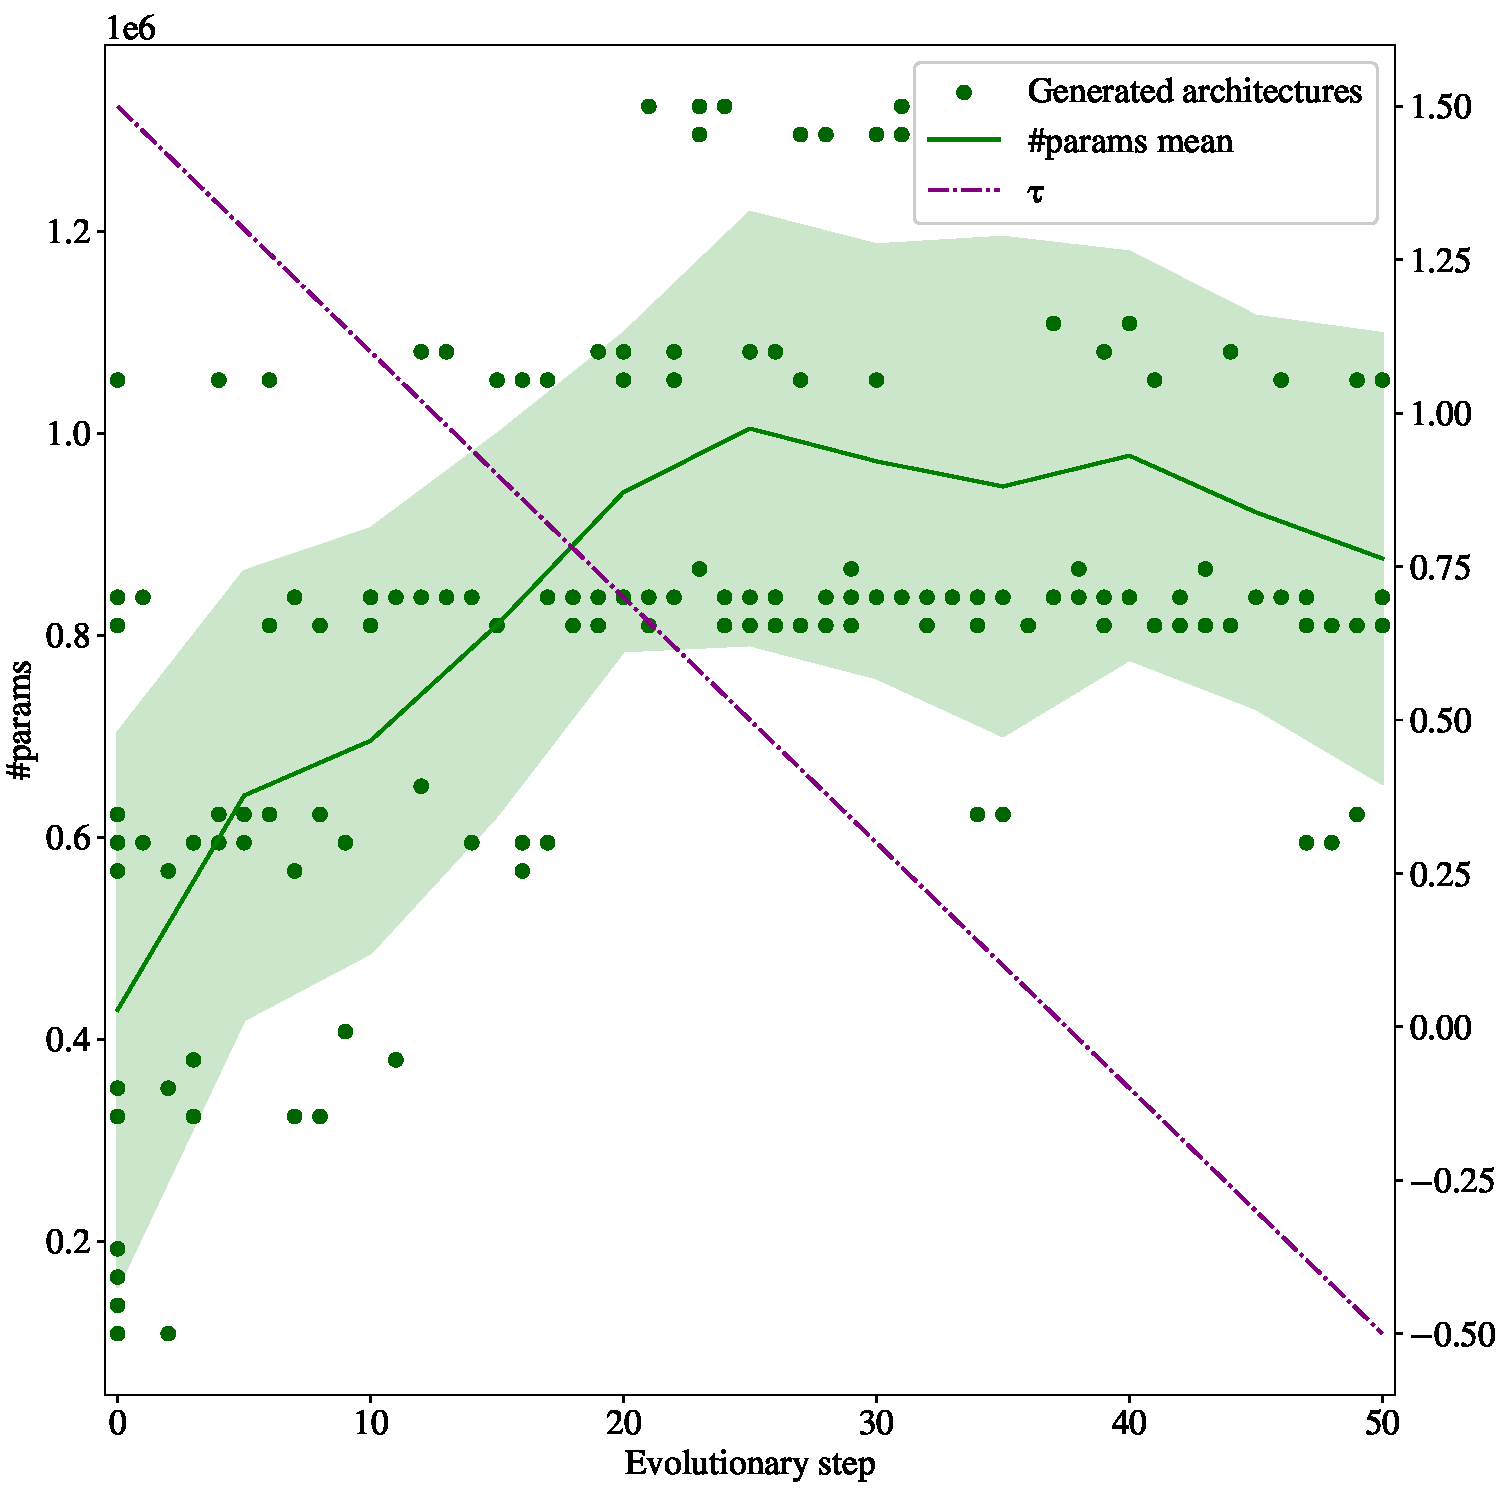
\includegraphics[width=\textwidth]{fig/params/params_adv_genetic_regparam_nasbench201_ImageNet16-120_meco_2025-04-30_17-00.pdf}
        \caption{ImageNet16-120}        \label{fig_params_meco_ImageNet16120}
    \end{subfigure}%

\end{adjustbox}
\caption{\centering Evolution of sampled architectures' parameter counts during genetic search with a parameter-based discriminator. The paired ZCP guiding the search is \texttt{meco}, which is usually biased towards overparameterized models. The average parameter count and its std error (in green) are constrained by the linear $\tau$ schedule during the search.}
\label{fig_params_meco}
\end{figure}

\subsection{Model size control}
\label{experiments_params}

To verify that the size of the models in the population is being meaningfully controlled by the ParaDis constraint, we plot the parameter counts of architectures sampled during the search. We present the results on three vision tasks in Fig.~\ref{fig_params_meco} with \texttt{meco}, a proxy heavily biased towards large model sizes, as the explorer metric. 

We observe three easily identifiable phases of the search corresponding to the linear schedule of $\tau$: at the start, the sizes of sampled architectures are pushed up by the explorer and the discriminator with positive $\tau$. Towards the middle, the parameter counts stagnate or increase slowly as the population stabilizes and $\tau$ approaches 0. At the end of the search, with negative $\tau$, the discriminator prevents parameter counts from increasing further, thus avoiding overparameterized regions. These results demonstrate that the discriminator properly controls the region of architecture sampling with respect to model size.

\section{Limitations and perspectives}
\label{limitations}

An important limitation of the family of zero-cost NAS methods is that, to the best of our knowledge, no universal solution exists. As observed in our experiments, no single ZCP is a clear cut above the others on every task, despite the similarities in domain and search space, although some metrics can be observed to perform better overall. Similarly, while the proposed ParaDis finds better architectures on average, it does not perform better on every task. Therefore, a major drawback of the literature remains the overabundance of choice available between proxy design, search algorithm design and hyperparameters. 

Additionally, while experimental results confirm the effectiveness of the genetic framework with the ParaDis discriminator, our proposed solution is merely a naive but effective approach. While the literature progresses rapidly on the topic of a proxy to guide the search towards better architectures, very little focus is given to proxies that select poor architectures to remove from the space. We hope that our insights will open this new question in the literature.

\section{Conclusion}
\label{conclusion}

In this work, we identify a fundamental limitation of zero-cost proxies (ZCPs) in neural architecture search (NAS): their difficulty in distinguishing among top-performing architectures within large search spaces. While effective globally, ZCPs tend to favor architectures with high parameter counts, reducing their discriminative power at the high-performance end. To address this, we introduce ParaDis, a generic and search space-agnostic approach that controls the parameter count distribution to remove this bias. By constraining the search region, ParaDis enables ZCPs to better focus on promising candidates. Experiments on NAS-Bench-201 and TransNAS-Bench-101 demonstrate consistent improvements in discovered architectures across diverse tasks. Our method’s robustness and versatility stem from its orthogonality to ZCP design and lack of assumptions on the search space. Overall, ParaDis advances zero-shot NAS by complementing ZCPs with an effective model size control mechanism.

%%%
%%%\subsubsection*{Acknowledgments}
%%%Use unnumbered third level headings for the acknowledgments. All
%%%acknowledgments, including those to funding agencies, go at the end of the paper.
%%%Only add this information once your submission is accepted and deanonymized.
%%%

\newpage

\bibliography{bibliography}
\bibliographystyle{tmlr}

\newpage

\appendix

\section{Search space encodings}
\label{apx_encodings}

In this section, we detail the encodings of the search spaces used for the experiments, largely based on the implementation from~\citet{krishnakumar2022bench}.

\subsection{NAS-Bench-201}

The genome encoding of architectures from the NB201 space~\citep{dong2020bench} is directly inferred from their graph-like cell structure. The cell is directly copied and stacked to form a complete network, therefore it is sufficient to encode a single cell. Each edge of the cell's graph is assigned to a genome position. The operation choices of the space (5 possible operations) are encoded into each position as a numerical value. With 6 edges in the graph, the resulting genome is a 6 values long string.

\subsection{TransNAS-Bench-101 Micro}

Due to being based directly on the same setting, the genome encoding of architectures for the TNB101-Micro space~\citep{duan2021transnas} is similar to the encoding for the NB201, with 6 edges and 4 operation choices.

\subsection{TransNAS-Bench-101 Macro}

The TNB101-Macro space~\citep{duan2021transnas} consists in a stack of 4 to 6 residual blocks where the locations of up to 4 downsamplings and up to 3 channel doublings can be chosen. It is therefore encoded as a string of 6 values, with each value assigned to one of the possible combinatorial choices: nothing, downsampling, double channels or downsampling+double channels. If the sampled architecture is smaller than the maximum size 6, the genome is padded with 0s to reach 6 values.

\section{Search space encodings}
\label{apx_encodings}

In this section, we detail the encodings of the search spaces used for the experiments, largely based on the implementation from~\citet{krishnakumar2022bench}.

\subsection{NAS-Bench-201}

The genome encoding of architectures from the NB201 space~\citep{dong2020bench} is directly inferred from their graph-like cell structure. The cell is directly copied and stacked to form a complete network, therefore it is sufficient to encode a single cell. Each edge of the cell's graph is assigned to a genome position. The operation choices of the space (5 possible operations) are encoded into each position as a numerical value. With 6 edges in the graph, the resulting genome is a 6 values long string.

\subsection{TransNAS-Bench-101 Micro}

Due to being based directly on the same setting, the genome encoding of architectures for the TNB101-Micro space~\citep{duan2021transnas} is similar to the encoding for the NB201, with 6 edges and 4 operation choices.

\subsection{TransNAS-Bench-101 Macro}

The TNB101-Macro space~\citep{duan2021transnas} consists in a stack of 4 to 6 residual blocks where the locations of up to 4 downsamplings and up to 3 channel doublings can be chosen. It is therefore encoded as a string of 6 values, with each value assigned to one of the possible combinatorial choices: nothing, downsampling, double channels or downsampling+double channels. If the sampled architecture is smaller than the maximum size 6, the genome is padded with 0s to reach 6 values.

\section{ZCP details}
\label{apx_zcp}

In this section, we present the definitions of each benchmarked ZCP based on theoretical insights and their implementation.

\subsection{\texttt{\#params}}

\texttt{\#params} is defined simply as the number of trainable parameters in the network. We directly use the network implementation to count its parameters without need for additional data.

\subsection{\texttt{jacov}}

\texttt{jacov} is introduced in~\citet{mellor2021neural} as the standalone method NASWOT then later renamed as \texttt{jacov} in~\citet{abdelfattah2021zero}. It is defined based on the covariance matrix of the Jacobian:
$$
C = cov(\nabla_w(\mathcal{L}))
$$
where $\mathcal{L}$ is the loss. The Jacobian is obtained by concatenation of the gradients of the model from a backward pass over a single batch of data. Then, \texttt{jacov} is constructed as a measure of the ability of the model to differentiate inputs in the batch:
$$
\texttt{jacov} = - \sum_{i=1}^n \left(log(\lambda^i) + \frac{1}{\lambda^i}\right)
$$
where $\lambda_1 \dots \lambda_n$ are the eigenvalues of $C$.

\subsection{\texttt{grad\_norm}}

\texttt{grad\_norm} is introduced by~\citet{abdelfattah2021zero} as a naive baseline for ZCPs. When the norm of the gradients of the model is higher, the model intuitively progresses faster in its parameter space, and is therefore easier to train.
$$
\texttt{grad\_norm} = \|\nabla_w(\mathcal{L}(m, w)\|_{\mathcal{F}}
$$

\subsection{\texttt{snip}, \texttt{grasp}, \texttt{synflow}}

\texttt{snip}~\citep{lee2018snip} \texttt{grasp}~\citep{wang2020picking} and \texttt{synflow}~\citep{tanaka2020pruning} are saliency metrics introduced in the pruning literature to determine the importance of specific parameters. They are aggregated over the entire network to provide a measure of the overall saliency of parameters in the model.

$$
\texttt{snip} = \sum_i^N |\frac{\partial \mathcal{L}}{\partial \theta_i} \odot \theta_i|
$$

$$
\texttt{grasp} = \sum_i^N -\left(H\frac{\partial \mathcal{L}}{\partial \theta_i}\right) \odot \theta_i
$$

$$
\texttt{synflow} = \sum_i^N |\frac{\partial \mathcal{L}}{\partial \theta_i} \odot \theta_i|
$$

All 3 metrics are summed over the $N$ layers of the network. $\theta_i$ are the trainable parameters at layer $i$, $\mathcal{L}$ is the loss and $\odot$ is the Hadamard product. In the case of \texttt{grasp}, the Hessian $H$ is computed via the $\mathcal{R}\{\cdot\}$ trick~\citep{pearlmutter1994fast}. \texttt{synflow} is similar to \texttt{snip}, but is data-agnostic as it does not compute over a batch of data, instead using a full matrix of 1 as input to estimate the synaptic flow.

\subsection{\texttt{fisher}}

\texttt{fisher} is introduced as a ZCP by~\citet{abdelfattah2021zero}. It is based on the aggregated sum of layerwise Fisher information~\citep{theis2018faster, turner2019blockswap} over the $N$ layers of the model:
$$
\texttt{fisher} = \sum_i^N \left( \frac{\partial \mathcal{L}}{\partial z_i} z_i \right)^2
$$
where $z_i$ is the aggregation of post-activations at layer $i$ and $\mathcal{L}$ is the loss.

\subsection{\texttt{ntk}}

\texttt{ntk} is introduced as a ZCP in the TE-NAS method~\citep{chen2021neural} where it is paired with the number of linear regions. It is defined as the condition number of the Neural Tangent Kernel (NTK)~\citep{jacot2018neural, lee2019wide, xiao2019disentangling}. Networks with lower condition number have better convergence property and trainability. We estimate the Neural Tangent Kernel following the TE-NAS estimation scheme:
$$
\Theta = \nabla_w(\mathcal{L}^T\nabla_w(\mathcal{L})
$$
where $\mathcal{L}$ is the loss and $w$ are the trainable parameters of the model. Considering the eigenvalues $\lambda_0 \dots \lambda_n$ of $\Theta$, we have:
$$
\texttt{ntk} =  \lambda_n / \lambda_0
$$

\subsection{\texttt{zen}}

\texttt{zen} is introduced in~\citet{lin2021zen} as a ZCP based on the noise error of the model and the statistics of the batch normalization layers (BN). Therefore, it is specific to search spaces that contain batch normalizations.

Let $x, \epsilon$ the inputs of \texttt{zen} sampled from a normal distribution $\mathcal{N}(0, 1)$. For model $f$ and hyperparameter $\alpha$, we have:
$$
\Delta = \mathbb{E}_{x, \epsilon}\|f(x) - f(x +\alpha\epsilon)\|_F
$$

And for all BN layer in the model, we define:
$$
\bar{\sigma} = \textstyle\sum_i log \left(\sqrt{\textstyle\sum_j^m \sigma_{i, j} ^2/m} \right)
$$
which considers the standard deviation $\sigma_{i,j}$ of BN layer $i$ at the $j$th out of $m$ channels.

Both parts of the metric are then summed:
$$
\texttt{zen} = log(\Delta) + \bar{\sigma}
$$

\subsection{\texttt{zico}}

\texttt{zico}~\citep{li2023zico} is introduced to evaluate the generalization capacity of architectures~\citep{keskar2016large, liang2017fisher} based on the statistics of the gradients:
$$
\texttt{zico} = \sum_{i=1}^N log \left( \sum_{\omega \in \theta_i} \frac{\mathbb{E\|\nabla_\omega\mathcal{L}\|}}{\sqrt{Var(\nabla_\omega\mathcal{L})}}\right)
$$
where $\theta_i$ are the trainable parameters at layer $i$ out of $N$ layers, and $\mathcal{L}$ is the loss.

\subsection{\texttt{meco}}

\texttt{meco}~\citep{jiang2023meco} is introduced based on similar insights as \texttt{zico} by noticing that the Pearson correlation matrix is closely related to the Gram matrix. Let the Pearson correlation matrix over the outputs of mode $f$ with input $X$:
$$
[\mathcal{P}(X)]_{i,j} = \frac{\mathbb{E}\|(f(X_i) - \mu_{f(X_i)})(f(X_j) - \mu_{f(X_j)})\|}{\sigma_{f(X_i)}\sigma_{f(X_j)}}
$$
where $\mu_x$ and $\sigma_x$ are the mean and standard deviation of $x$, respectively. \texttt{meco} is then computed based on the minimum eigenvalue $\lambda_{min}$ of the Pearson correlation matrix:
$$
\texttt{meco} = \textstyle\sum_{i=1}^N \lambda_{min}(\mathcal{P}(X))
$$

\subsection{\texttt{swap}}

\texttt{swap}~\citep{peng2024swap} is a reframing of the concept of linear regions partition in the latent space of the network to measure the expressivity of the network~\citep{raghu2017expressive, xiong2020number, chen2021neural}.

The set of sample-wise activation patterns of the network is gathered as:
$$
\hat{\mathbb{A}}_{\theta} = \left\{ \mathds{1} (p_s^{(v)})_{s=1}^S, v\in\{1, \dots ,V\}\right\}
$$
where $p_s^{(v)}$ is the post-activation of sample $s$ at value $v$. $\hat{\mathbb{A}}_{\theta}$ contains the one-hot encodings of all activation patterns obtained in the network for the samples in batch $S$.

\texttt{swap} is then equal to the number of activation patterns, which is the cardinal of the set:
$$
\texttt{swap} = |\hat{\mathbb{A}}_{\mathcal{\theta}}|
$$

\section{More details about the Spearman correlation benchmarks}
\label{apx_benchmark_details}

In the main paper, confidence intervals for the Spearman correlation benchmarks are omitted to keep the table readable. The displayed value is averaged over 3 seeds. In the following tables we present the Spearman correlation for both the full space setting and the top 1\% with $1\sigma$ error.

\begin{figure}[H]
\begin{adjustbox}{width=\linewidth}
    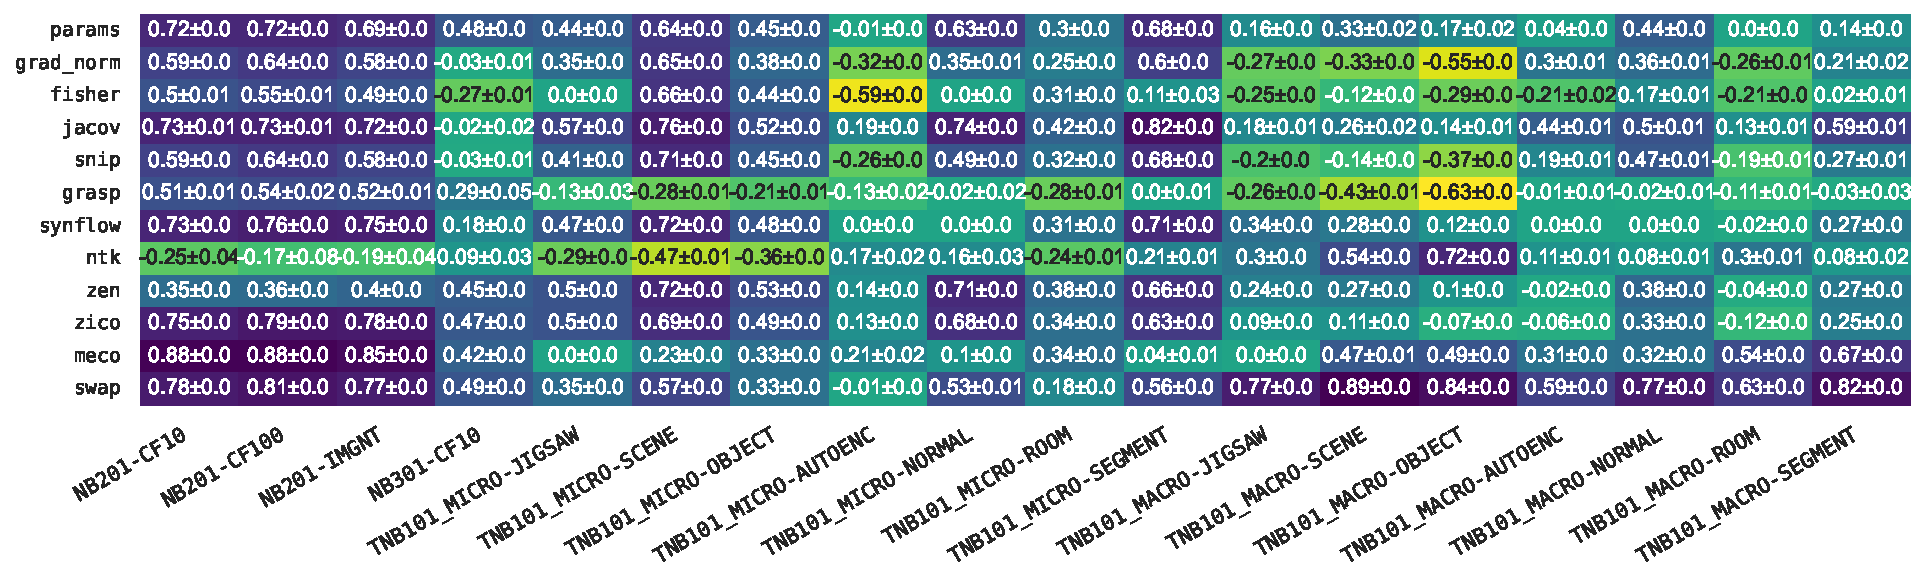
\includegraphics[width=\textwidth]{fig/benchmarks/zcp_corr_std.pdf}
\end{adjustbox}
\caption{\centering Spearman rank correlations of various ZCPs on the NAS-Bench-201, NAS-Bench-301 and TransNAS-Bench-101 benchmarks. Spearman was computed over 3 seeds against the entire search space.}
\label{fig_bench_corr_full}
\end{figure}

\begin{figure}[H]
\begin{adjustbox}{width=\linewidth}
    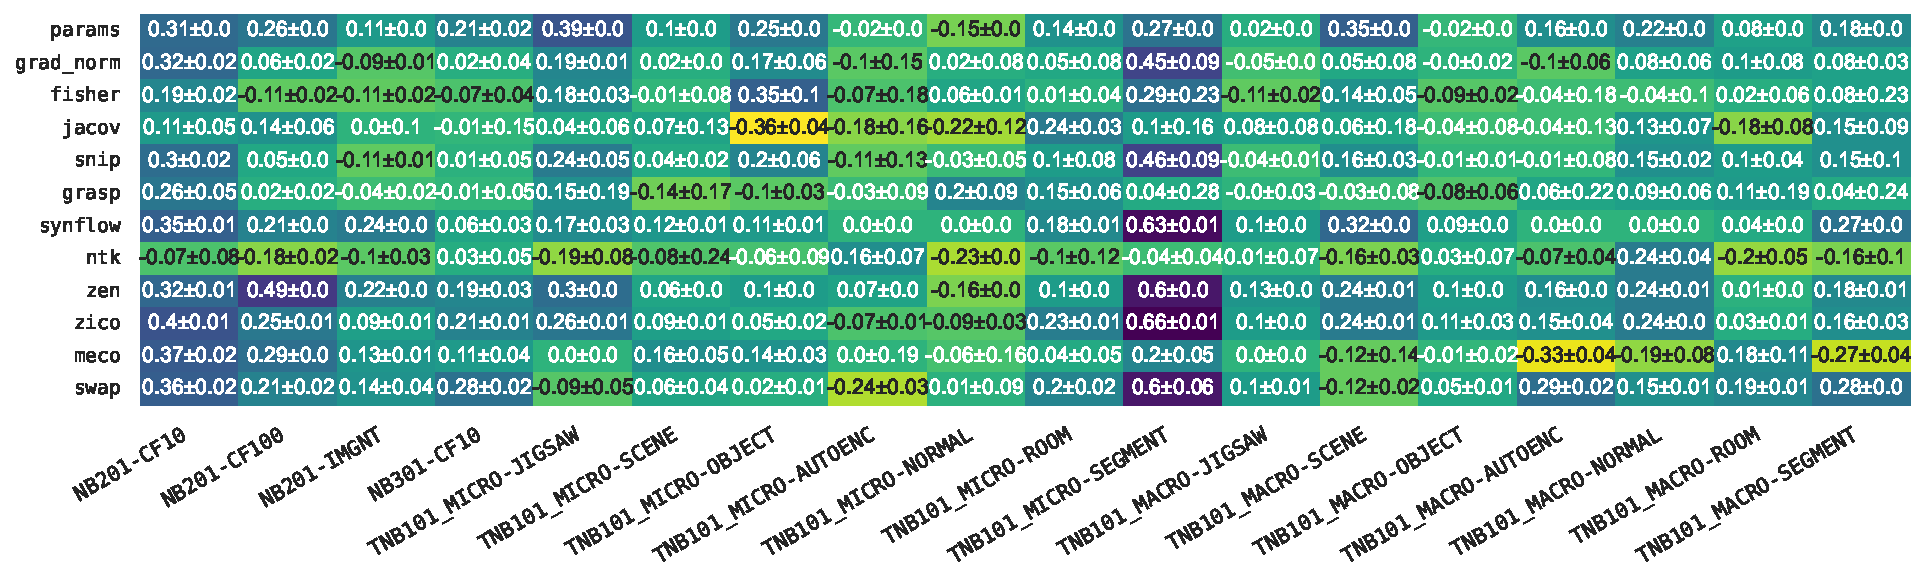
\includegraphics[width=\textwidth]{fig/benchmarks/zcp_corr_top1pct_std.pdf}
\end{adjustbox}
\caption{\centering Spearman rank correlations of various ZCPs on the NB201, NB301 and TNB101 benchmarks. Spearman was computed on 3 seeds against the top 1\% architectures in the space.}
\label{fig_bench_corr_full}
\end{figure}

\section{Full ParaDis algorithm}
\label{apx_algorithm}

\begin{algorithm}[H]
\caption{\underline{\textbf{Para}}meter \underline{\textbf{Dis}}tribution Shift NAS (\textbf{ParaDis})}
\label{alg_paradis}
\begin{algorithmic}[1]
\Require: population size $P$, sample size $p < P/2$, number of generations $N$, evolution steps per generation $S$, zero-cost metric $\mathcal{M}$, temperature schedule $[\tau_0, \tau_1, \dots, \tau_N]$
\State $population \gets \emptyset$
\While {$population.size < P$}
\State Randomly sample $arch$ from the space
\State $arch.score \gets \mathcal{M}(arch)$
\State $arch.params \gets CountParams(arch)$
\State Add $arch$ to $population$
\EndWhile
\State $\mu$, $\sigma \gets Mean(population.params), STD(population.params)$
\For {$arch$ in $population$}
\State $arch.\Phi \gets e^{-(\frac{arch.params - (\mu + \tau_0 \sigma)}{\sigma})^2}$
\EndFor
\For {$n=1,2,\dots,N$}
\State $\tau \gets \tau_n$
\For {$s=1,2,\dots S$}
\State $candidates_A$, $candidates_B \gets p$, $p$ random $archs$ of $population$
\State $candidates_C \gets$ all remaining $archs$ in $population$
\For {$candidates_A$, $candidates_B$}
\State $discarded \gets$ worst $arch$ by $\Phi$
\State $parent \gets$ best $arch$ by $arch.score$ except $discarded$
\State $child \gets Mutate(parent)$
\State $child.score \gets \mathcal{M}(child)$
\State $child.params \gets CountParams(child)$
\State Replace $discarded$ with $child$ in $population$
\EndFor
\State $discarded_C \gets$ worst $arch$ by $\Phi$ in $candidates_C$
\State $child_C \gets Crossover(parent_A, parent_B)$
\State $child_C.score \gets \mathcal{M}(child_C)$
\State $child_C.params \gets CountParams(child_C)$
\State Replace $discarded_C$ with $child_C$ in $population$
\EndFor
\State $\mu$, $\sigma \gets Mean(population.params), STD(population.params)$
\For {$arch$ in $population$}
\State $arch.\Phi \gets e^{-(\frac{arch.params - (\mu + \tau \sigma)}{\sigma})^2}$
\EndFor
\EndFor
\end{algorithmic}
\end{algorithm}

\end{document}
